\documentclass[journal]{IEEEtran}

\usepackage{cite}
\usepackage{amsmath,amssymb,amsfonts}
\usepackage{algorithmic}
\usepackage{algorithm}
\usepackage{graphicx}
\usepackage{textcomp}
\usepackage{xcolor}
\usepackage{booktabs}
\usepackage{multirow}
\usepackage{url}
\usepackage{array}
\usepackage{subcaption}
\usepackage{enumitem}
\setlist{noitemsep,topsep=2pt,parsep=0pt,partopsep=0pt}
\usepackage{balance}

\def\BibTeX{{\rm B\kern-.05em{\sc i\kern-.025em b}\kern-.08em
    T\kern-.1667em\lower.7ex\hbox{E}\kern-.125emX}}

\newtheorem{theorem}{Theorem}
\newtheorem{lemma}{Lemma}
\providecommand{\IEEEQED}{\hfill$\blacksquare$}
\ifdefined\proof\else
\newenvironment{proof}{\begin{IEEEproof}}{\end{IEEEproof}}
\fi

\setlength{\textfloatsep}{5pt plus 1pt minus 1pt}
\setlength{\floatsep}{4pt plus 1pt minus 1pt}
\setlength{\intextsep}{4pt plus 1pt minus 1pt}
\setlength{\dbltextfloatsep}{5pt plus 1pt minus 1pt}
\setlength{\dblfloatsep}{4pt plus 1pt minus 1pt}
\setlength{\abovecaptionskip}{2pt}
\setlength{\belowcaptionskip}{2pt}
\setlength{\abovedisplayskip}{3pt plus 1pt minus 1pt}
\setlength{\belowdisplayskip}{3pt plus 1pt minus 1pt}
\setlength{\abovedisplayshortskip}{2pt plus 1pt minus 1pt}
\setlength{\belowdisplayshortskip}{2pt plus 1pt minus 1pt}

\begin{document}

\title{Crypto-Induced Latency Denial of Service in IEC~61850 Substation Communications: Cyber-Physical Impact Analysis, Priority Admission Defense, and Post-Quantum Evaluation}

\author{Sapna~Vikram~Mewundi,
        Prajwal~Chowdary~M.,
        and~Prasad~B.~Honnavalli%
\thanks{This work was supported by the Department of Computer Science and Engineering, PES University, Bengaluru, India. \textit{(Corresponding author: Sapna Vikram Mewundi.)}}%
\thanks{Sapna Vikram Mewundi is with the Department of Computer Science and Engineering, PES University, Bengaluru, 560085, India (e-mail: sapnavm@pes.edu).}%
\thanks{Prajwal Chowdary M. and Prasad B. Honnavalli are with the Department of Computer Science and Engineering, PES University, Bengaluru, 560085, India (e-mail: prajwalchowdary@pes.edu; prasadhb@pes.edu).}%
}

\markboth{IEEE Transactions on Smart Grid}%
{Mewundi \MakeLowercase{\textit{et al.}}: Crypto-Induced Latency Denial of Service in IEC 61850 Substation Communications}

\maketitle

\begin{abstract}
IEC~62351-6 secures IEC~61850 GOOSE trip messages with cryptographic authentication, but asymmetric and post-quantum (PQC) signatures impose serialized verification latency on resource-constrained Intelligent Electronic Devices (IEDs). We identify Crypto-Induced Latency Denial of Service (CIL-DoS): any receiver that verifies every frame before filtering is floodable, and for asymmetric/PQC profiles---on which we focus---an adversary can saturate the verification queue with syntactically valid but invalid GOOSE frames, delaying trips past the 3\,ms Class~P2/P3 deadline at a flood rate orders of magnitude below that needed for symmetric MACs. We (i)~formalize CIL-DoS with $M/M/1$ and $M/D/1$ models and link the delay to generator transient stability via a numerically integrated single-machine swing equation (critical clearing time $201.6$\,ms), ANSI~50BF breaker-failure escalation, and transformer $I^2t$ stress; (ii)~show buffer bloat and parallel workers both retain 100\% deadline failure on a service-time-calibrated Cortex-A9 relay emulation; (iii)~propose the Priority Queue Admission Controller (PQAC), prove its stability ($\rho_H<1$), and measure (5 reps) a $3{,}140\times$ mean-latency reduction on the emulated relay ($2{,}388$\,ms$\to$$760\,\mu$s, P99 $1.12$\,ms, $0.00\%$ deadline miss) and $1{,}333\times$ on the host; (iv)~show by measured ablation that rate-anomaly dropping is decisive under single-source floods while priority isolation becomes necessary under multi-source (random-MAC) floods, and that spoofed-MAC floods cause $\approx 95\%$ \emph{trip loss} that only switch port-security/MACsec can prevent; and (v)~validate the cryptographic costs on real silicon (ESP32: RSA-2048 verify $980\,\mu$s, ECDSA-P256 verify $310$\,ms). A NIC-level eBPF/XDP pre-filter is specified as complementary future work. All artifacts are open-sourced.
\end{abstract}

\begin{IEEEkeywords}
Substation automation, IEC 61850 GOOSE, IEC 62351-6, smart grid cyber-physical security, power system stability, post-quantum cryptography, ML-DSA, priority queueing, eBPF/XDP.
\end{IEEEkeywords}

%% ================================================================
%%  SECTION I: INTRODUCTION
%% ================================================================
\section{Introduction}
\label{sec:intro}
\IEEEPARstart{M}{odern} electrical power grids increasingly depend on Substation Automation Systems (SAS) to isolate physical electrical faults within milliseconds, preventing cascading blackouts that inflict billions of dollars in economic damages annually~\cite{huseinovic2020dos}. The International Electrotechnical Commission (IEC)~61850 standard defines the communication architecture for digital substations, replacing copper point-to-point wiring with high-speed Ethernet process buses~\cite{iec61850}.

Among its core communication protocols, Generic Object Oriented Substation Events (GOOSE) carry the most time-critical protection data: trip signals transmitted between Intelligent Electronic Devices (IEDs) and circuit breaker controllers. For Performance Class~P2/P3 high-voltage applications, IEC~61850 caps the total end-to-end transmission delay at \textbf{3 milliseconds (ms)}~\cite{iec61850}. Exceeding this real-time deadline during an electrical short-circuit can cause severe generator instability, explosive transformer failures, or cascading grid collapse.

\subsection{The Security-Safety Paradox}
Originally, GOOSE messages operated as unauthenticated Layer~2 Ethernet multicast frames (EtherType \texttt{0x88B8}), rendering substations vulnerable to packet spoofing, replay, and unauthorized trip injection~\cite{schuster2017goose, hong2014cyber}. To address these vulnerabilities, the IEC introduced the \textbf{IEC~62351-6} standard~\cite{iec62351}, specifying cryptographic authentication profiles: digital signatures (RSA-2048, ECDSA-P256) and symmetric authentication codes (HMAC-SHA256).

Recognizing the strict 3\,ms Class~P2/P3 latency requirement, IEC~62351-6 Edition 2 recommends symmetric MACs (HMAC-SHA256 / AES-GMAC) as the primary profile for routine GOOSE multicast. However, symmetric group keys lack cryptographic non-repudiation: because all IEDs on the process bus share the identical key, a single compromised peripheral device exposes the key, enabling arbitrary trip forgeries without detection. In contrast, asymmetric digital signatures and post-quantum cryptography (PQC) guarantee non-repudiation: each publisher holds a unique private key. Yet asymmetric verification is computationally expensive and serialized on embedded IED processors. We note that CIL-DoS, as a \emph{queueing} attack, targets relays that are fast enough to meet the 3\,ms budget in the absence of attack (Cortex-A9/Atom class and above, Section~\ref{sec:architecture_queueing}); the slowest microcontroller cores (Cortex-R5/M4) already exceed the budget on a single verification and are out of scope. Because invalid signatures cannot be detected prior to full mathematical verification, every incoming frame consumes scarce processor cycles. This creates what we term the \emph{security-safety paradox}: cryptographic authentication introduces per-frame computational overhead that can be exploited to violate real-time safety deadlines. The effect is a matter of degree: on our embedded test device (ESP32, Section~\ref{sec:architecture_queueing}) even symmetric HMAC/GMAC verifies at only $\sim$4{,}400--6{,}000\,fps, so a flood above a few thousand pps can in principle saturate it; asymmetric RSA verify runs at $\sim$1{,}000\,fps and software ECDSA at $\sim$3\,fps, lowering the required flood rate by one to four orders of magnitude. We therefore focus CIL-DoS on the asymmetric and PQC profiles, where the attack is dramatically cheaper, while noting that a verify-every-frame symmetric receiver on a slow core is not immune.

\subsection{Research Problem and Positioning}
We identify an exploitable attack vector: \textbf{Crypto-Induced Latency Denial of Service (CIL-DoS)}. An adversary with process bus access floods syntactically valid GOOSE frames bearing random, invalid signatures. The receiver accepts packets at wire speed ($>$100,000\,pps), while the verifier processes them at orders-of-magnitude lower rates ($\sim$1,745\,pps for RSA-2048 on embedded relays, $\sim$29,689\,pps on high-speed hosts). As the verification queue saturates, legitimate protection commands queue behind malicious traffic and miss the 3\,ms hard real-time safety deadline.

\textbf{Adversary Positioning (where PQAC adds value).} A process-bus attacker who can inject frames at line rate can, in principle, also \emph{spoof} a legitimate publisher's source MAC; against such an attacker no application-layer admission scheme---PQAC included---can separate attacker from victim, and our own evaluation (Section~\ref{sec:spoof_eval}) measures a $\approx 95\%$ collapse in trip delivery under shared-MAC spoofing. PQAC is therefore explicitly \emph{not} positioned as a spoofing defense. Its value lies in the large and operationally common band where the Layer-2 \emph{identity} is already protected---switch port-to-MAC binding (port security) or MACsec---so that an adversary (a compromised or tapped device behind that control) can still mount a high-rate flood under its \emph{own} or an unknown MAC, but cannot impersonate an authorized publisher. In that band, which covers the vast majority of brownfield digital substations once basic port security is enabled, cross-MAC spoofing is blocked at the switch while same-MAC/unknown-MAC crypto floods pass straight through to the verifier---and it is precisely there that PQAC restores the deadline. We make this scoping explicit throughout and treat unprotected-identity spoofing as a stated boundary, not a solved case.

\textbf{Scope Clarification:} The objective of this paper is \emph{not} to propose a new transmission protection algorithm or modify relay tripping curves. Rather, we address a foundational cyber-physical communication challenge: quantifying how cryptographic overhead in digital substation networks induces queue saturation, how that communication delay propagates across physical power systems, and how real-time admission control can safeguard standard protection schemes.

\subsection{Key Contributions}
The major contributions of this work are:
\begin{enumerate}[leftmargin=*,noitemsep,topsep=1pt]
    \item \textbf{CIL-DoS Formalization and Cyber-Physical Modeling:} We formalize CIL-DoS via $M/M/1$ and $M/D/1$ queueing models and quantify physical consequences: rotor angle divergence exceeding Critical Clearing Time ($t_{\text{crit}} \approx 201.6$\,ms base, $\approx 120$\,ms in low-inertia grids), ANSI 50BF breaker failure escalation ($t_{\text{clear}} \approx 216$\,ms), and a $6.25\times$ surge in transformer $I^2 t$ thermal energy under 350\,ms backup clearance ($3.6\times$ under 200\,ms 50BF clearance).
    \item \textbf{Decoupled Subscriber Architecture:} We implement a two-thread C subscriber architecture separating wire-speed frame ingestion from serialized cryptographic verification.
    \item \textbf{Evaluation of Na\"ive Countermeasures:} We demonstrate that increasing queue depth 4$\times$ inflates latency by 4$\times$ (to 552\,ms on the measured host and a measured 8,898\,ms on the emulated relay), while 4 parallel verification workers still yield 100\% deadline failure on resource-constrained embedded relays.
    \item \textbf{Priority Queue Admission Controller (PQAC):} We design PQAC, prove queue stability ($\rho_H < 1$) and delay isolation, and establish an algorithmic worst-case bound of 1.197\,ms on embedded relays. Its \emph{novel} core is two GOOSE-semantic mechanisms---(a)~RFC~1982 serial-arithmetic \texttt{stNum} \emph{plausibility gating} that admits a state transition to the protection class only within a bounded window, and (b)~\emph{verify-before-commit}, which updates the trusted state counter \emph{only} after signature verification, preventing state-poisoning and trip-suppression; the surrounding per-source policing and strict priority are a correct composition of known mechanisms tuned to the 3\,ms regime. Measured over 5 reps, PQAC achieves a $3{,}140\times$ mean-latency reduction on the emulated Cortex-A9 relay (2{,}388\,ms$\to$760\,$\mu$s, 0.00\% miss) and $1{,}333\times$ on the host (100\,ms$\to$75\,$\mu$s, 0.17\% miss, a cold-start artifact), validated via a measured component ablation.
    \item \textbf{NIST Post-Quantum Cryptography Evaluation:} We benchmark NIST PQC standards (ML-DSA-44, ML-DSA-87, SLH-DSA, FALCON-512) for IEC~61850, revealing that hash-based SLH-DSA exhibits an unviable 295--597\,ms signing latency and 7.8\,kB jumbo frame requirement, whereas lattice-based verification is sub-millisecond on the host and is effectively shielded by PQAC, with the caveat that ML-DSA-87 projects to $\approx 2.4$\,ms on a Cortex-A9---approaching the Theorem~3 precondition.
    \item \textbf{Layered Defense Specification:} We evaluate the application-layer PQAC across 48 controlled experiments and \emph{specify} (as future implementation work) a complementary NIC-level eBPF/XDP pre-filter. All testbed artifacts and scripts are open-sourced.
\end{enumerate}

%% ================================================================
%%  SECTION II: BACKGROUND AND RELATED WORK
%% ================================================================
\section{Background and Related Work}
\label{sec:background}

\subsection{IEC 61850 GOOSE Protocol Architecture}
GOOSE operates directly over Layer~2 Ethernet (EtherType \texttt{0x88B8}), avoiding Layer~3/4 protocol overhead. The ASN.1 BER-encoded protocol data unit contains:
(1)~\texttt{gocbRef} (control block reference), (2)~\texttt{datSet} (dataset name), (3)~\texttt{appID} (application identifier), (4)~\texttt{stNum} (state counter incremented upon state transitions such as breaker trips), (5)~\texttt{sqNum} (sequence counter incremented on every retransmission), and (6)~\texttt{allData} (trip/measurement status).
Following a trip, GOOSE uses burst retransmissions: $T_0 = 1$\,ms, doubling ($2, 4, 8$\,ms) up to a heartbeat $T_{\max} = 1,000$\,ms.

\subsection{IEC 62351-6 Cryptographic Profiles and PQC Candidates}
Table~\ref{tab:crypto_taxonomy} categorizes the cryptographic profiles evaluated in this work, spanning standard IEC~62351-6 mechanisms and emerging NIST Post-Quantum Cryptography (PQC) standards.

\begin{table}[t]
\centering
\caption{Cryptographic Algorithm Evaluation Taxonomy}
\label{tab:crypto_taxonomy}
\scriptsize
\resizebox{\columnwidth}{!}{%
\begin{tabular}{llcc}
\toprule
\textbf{Algorithm} & \textbf{Cryptographic Class} & \textbf{IEC 62351-6 Status} & \textbf{Evaluation Role} \\
\midrule
RSA-2048    & Asymmetric (PKI)     & Standard Profile & Classical Asymmetric Baseline \\
ECDSA-P256  & Elliptic Curve (ECC) & Standard Profile & Compact Signature Baseline \\
HMAC-SHA256 & Symmetric Key (MAC)  & Standard Profile & Symmetric Performance Limit \\
\midrule
ML-DSA-44   & Lattice-based (FIPS 204) & PQC Candidate & Primary NIST Quantum-Safe \\
ML-DSA-87   & Lattice-based (FIPS 204) & PQC Candidate & High-Security Quantum-Safe \\
SLH-DSA     & Hash-based (FIPS 205)    & PQC Candidate & Stateless Hash-Based Baseline \\
FALCON-512  & Lattice-based (NIST)     & PQC Candidate & Low-Latency Compact Signature \\
\bottomrule
\end{tabular}%
}
\end{table}

\subsection{Related Work and Research Gaps}
Prior research on substation cybersecurity falls into five main categories:
\begin{enumerate}[leftmargin=*,noitemsep,topsep=1pt]
    \item \textbf{GOOSE Protocol Exploits:} Schuster \textit{et al.}~\cite{schuster2017goose} and Hoyos \textit{et al.}~\cite{hoyos2012real} showed unauthenticated GOOSE can be spoofed to trip breakers. Yang \textit{et al.}~\cite{yang2013cyber} mapped substation cyber surfaces. These works established authentication needs but omitted overhead as an attack surface.
    \item \textbf{IEC 62351-6 Performance Overhead:} Farooq \textit{et al.}~\cite{farooq2019goose} evaluated the RSA probabilistic signature scheme and Hussain \textit{et al.}~\cite{kabir2020goose} analyzed message-authentication-code algorithms for GOOSE, noting that verification delays can approach real-time limits, but both analyzed only benign operation without adversarial traffic.
    \item \textbf{Smart Grid Denial of Service:} Huseinovi\'{c} \textit{et al.}~\cite{huseinovic2020dos} and Khan \textit{et al.}~\cite{khan2021survey} surveyed network-layer flooding. Whereas the denial-of-service potential of signature-verification load has been noted in V2X networks~\cite{biswas2014dos}, substations feature unique constraints: sub-3\,ms deadlines, static bay topologies, and unrouted Layer~2 multicast.
    \item \textbf{Substation Intrusion Detection:} Ustun \textit{et al.}~\cite{hussain2019goose} and Quincozes \textit{et al.}~\cite{quincozes2021survey} studied substation intrusion detection; however, passive detection cannot prevent queues from filling in real time.
    \item \textbf{Post-Quantum Smart Grid Security:} Empirical timing evaluations of NIST FIPS 204/205 under IEC~61850 real-time constraints have remained absent. All artifacts are available at \url{https://github.com/gridpulse-project/cil-dos-artifacts}.
\end{enumerate}

Table~\ref{tab:related_work} contrasts our work with prior research, highlighting our contribution in connecting cryptographic queue saturation with cyber-physical grid stability.

\begin{table}[t]
\centering
\caption{Comparison with Related Research}
\label{tab:related_work}
\scriptsize
\resizebox{\columnwidth}{!}{%
\begin{tabular}{lcccc}
\toprule
\textbf{Study} & \textbf{Attack Vector} & \textbf{Crypto Eval.} & \textbf{Queue Model} & \textbf{Physical Consequence} \\
\midrule
Schuster \textit{et al.}~\cite{schuster2017goose} & Spoofing & None & No & Breaker misoperation \\
Farooq \textit{et al.}~\cite{farooq2019goose}   & Overhead & RSA-PSS & No & Latency measurement \\
Huseinovi\'{c} \textit{et al.}~\cite{huseinovic2020dos}     & Network DoS & None & Heuristic & Communication loss \\
Ustun \textit{et al.}~\cite{ustun2019novel}       & Replay/FDI & MAC & No & Protection blinding \\
\textbf{This Work}                                & \textbf{CIL-DoS} & \textbf{RSA/PQC} & \textbf{Theorems 1--3} & \textbf{CCT / 50BF / $I^2 t$} \\
\bottomrule
\end{tabular}%
}
\end{table}

%% ================================================================
%%  SECTION III: THREAT MODEL & CYBER-PHYSICAL IMPACT
%% ================================================================
\section{Threat Model and Cyber-Physical Impact}
\label{sec:threat_model}

\subsection{Network Model and Attacker Capabilities}
We consider a digital substation process bus connecting merging units, protection relays, and circuit breaker controllers via Layer~2 Ethernet. An adversary gains Layer~2 process bus access via an infected engineering workstation, compromised gateway, or physical Ethernet tap~\cite{cherepanov2017industroyer}. The attacker cannot forge valid private keys, but can inject arbitrary Layer~2 Ethernet frames at line rate.

Standard process buses operate on 100BASE-FX (100\,Mbps) or 1000BASE-SX (1\,Gbps) optical Ethernet. For standard 350-byte GOOSE frames (370 wire bytes including preamble, SFD, and inter-frame gap), maximum physical link capacity is $100 \times 10^6 / (370 \times 8) = 33{,}783$\,pps ($\approx 33.8$\,kpps) on 100BASE-FX and $1{,}000 \times 10^6 / (370 \times 8) = 337{,}837$\,pps ($\approx 337.8$\,kpps) on 1000BASE-SX. For post-quantum GOOSE frames carrying larger signatures, physical line rates are further constrained: ML-DSA-44 ($\approx 2{,}520$ wire bytes) is physically capped at $49{,}600$\,pps on 1\,Gbps links, while SLH-DSA ($\approx 7{,}956$ wire bytes) is physically capped at $15{,}700$\,pps.

Crucially, CIL-DoS does \emph{not} require saturating physical network bandwidth or exceeding line rates. On an embedded protective relay (ARM Cortex-A9, $\mu = 1{,}745$\,fps), an attacker injecting a modest flood of just 5,000 to 10,000\,pps consumes only $\approx 14\text{--}28$\,Mbps ($<28\%$ of 100\,Mbps line capacity). The physical link remains over 70\% idle and uncongested, yet the cryptographic verification queue saturates monotonically ($\rho = 2.86\text{--}5.73 \gg 1$), delaying legitimate trip commands into seconds. While our virtualized testbed evaluates throughput up to 100K and 500K\,pps to benchmark the computational ceiling of the software ingestion pipeline across multi-gigabit virtual interfaces, real-world process buses are bounded by these physical line capacities, under which CIL-DoS readily achieves queue saturation.

\subsection{CIL-DoS Attack Dynamics}
The attacker transmits syntactically compliant GOOSE frames with pseudo-random signature bytes at rate $\lambda_{\text{atk}}$. Because the receiver cannot distinguish valid signatures from invalid signatures prior to full cryptographic execution, every frame enters the verification queue. When $\lambda_{\text{atk}} > \mu$ (verifier service rate), the queue accumulates monotonically, and legitimate trip frames experience severe queueing delay $W_q$.

\subsection{Cyber-Physical Impact on Power Grid Stability}
\label{sec:cyber_physical}
In power transmission grids, a GOOSE trip delay is not merely a communication delay; it directly cascades into electromechanical instability and severe protection selectivity loss:

\subsubsection{Rotor Angle Stability and Critical Clearing Time (CCT)}
The transient electromechanical swing equation of a synchronous generator during a severe three-phase bus fault is governed by~\cite{kundur1994power}:
\begin{equation}
\frac{2H}{\omega_s} \frac{d^2 \delta(t)}{dt^2} = P_m - P_e(\delta) = P_m - P_{\max}^{\text{fault}} \sin(\delta(t)),
\label{eq:swing}
\end{equation}
where $H$ is the generator inertia constant ($3\text{--}5$\,s), $\omega_s = 2\pi f_0 = 120\pi$\,rad/s, $\delta(t)$ is the rotor electrical angle, $P_m$ is mechanical shaft power, and $P_e$ is electrical power transfer. During a bolted three-phase fault near the substation, $P_{\max}^{\text{fault}} \approx 0$, yielding accelerating power $P_a \approx P_m$. Integrating~\eqref{eq:swing} with initial rotor angle $\delta_0$ yields:
\begin{equation}
\delta(t) = \delta_0 + \frac{\omega_s P_m}{4H} t^2.
\end{equation}
The Critical Clearing Time (CCT, $t_{\text{crit}}$) defines the maximum allowable fault duration before $\delta > \delta_{\text{cr}}$, beyond which synchronism with the infinite bus is irreversibly lost.

\textit{SMIB Benchmark Case Study:} Consider a standard Single-Machine Infinite-Bus (SMIB) benchmark system~\cite{kundur1994power} with generator parameters: $H = 4.0$\,s, transient reactance $X_d' = 0.25$\,p.u., mechanical input $P_m = 0.8$\,p.u., and nominal operating angle $\delta_0 = 32.5^\circ = 0.5672$\,rad, giving pre-fault power transfer capability $P_{\max} = P_m / \sin \delta_0 = 1.4888$\,p.u. For a bolted fault ($P_e = 0$) cleared by restoring the line without topology change, the Equal-Area Criterion equates accelerating area $A_{\text{acc}} = P_m(\delta_{\text{cr}} - \delta_0)$ and decelerating area $A_{\text{dec}} = \int_{\delta_{\text{cr}}}^{\pi - \delta_0} (P_{\max}\sin\delta - P_m)d\delta$, yielding:
\begin{equation}
\cos \delta_{\text{cr}} = \sin \delta_0 (\pi - 2\delta_0) - \cos \delta_0.
\label{eq:eac}
\end{equation}
Substituting $\delta_0 = 32.5^\circ$ into~\eqref{eq:eac} yields $\cos \delta_{\text{cr}} = 0.5373(2.0071) - 0.8434 = 0.2350$, giving critical clearing angle $\delta_{\text{cr}} = \arccos(0.2350) \approx 76.4^\circ$ and allowable angular advance $\Delta \delta = 76.4^\circ - 32.5^\circ = 43.9^\circ$. Rotor acceleration in degrees is:
\begin{equation}
\delta(t) = 32.5^\circ + 1{,}080\,t^2 \text{ [deg]}.
\end{equation}
The corresponding Critical Clearing Time is:
\begin{equation}
t_{\text{crit}} = \sqrt{\frac{76.4^\circ - 32.5^\circ}{1{,}080}} = \sqrt{0.04065} \approx 201.6\,\text{ms} \approx 200\,\text{ms}.
\end{equation}
In stressed, heavily loaded, or low-inertia inverter-based grids ($H = 2.5$\,s, $P_m = 0.95$\,p.u., acceleration $\alpha = 2{,}052^\circ/\text{s}^2$, $\delta_{\text{cr}} = 69.4^\circ$), $t_{\text{crit}}$ compresses to $\approx 120$\,ms.
Under nominal primary protection, total clearance time is $t_{\text{clear}} = t_{\text{relay}} + t_{\text{GOOSE}} + t_{\text{mech}} \approx 15 + 1.2 + 40 = 56.2$\,ms, which operates safely well below $t_{\text{crit}}$.

\subsubsection{Breaker Failure (ANSI 50BF) and Complete Clearing Timeline}
In high-voltage substations, an unmitigated CIL-DoS attack delaying primary GOOSE trip delivery beyond 2\,s triggers severe \emph{backup protection escalation}:
\begin{enumerate}[leftmargin=*,noitemsep,topsep=1pt]
    \item \textbf{ANSI 50BF Escalation on Flooded Bus:} Concurrently with primary trip initiation, relays start an ANSI 50BF Breaker Failure timer ($t_{\text{50BF}} \approx 150\text{--}200$\,ms). Because the primary breaker never receives the queued GOOSE trip, fault current persists past $t_{\text{50BF}}$, dispatching backup trips to adjacent circuit breakers. Total physical clearing time is:
    \begin{equation}
    t_{\text{clear}} = t_{\text{relay}} + t_{\text{50BF}} + t_{\text{comm}} + t_{\text{mech}} \approx 216.2\,\text{ms},
    \end{equation}
    where $t_{\text{relay}} \approx 15$\,ms, $t_{\text{mech}} \approx 40\text{--}60$\,ms (2.5--3.5 cycles at 60\,Hz). Under \emph{nominal} (unflooded) communications ($t_{\text{comm}} \approx 1.2$\,ms), this already yields $15 + 150 + 1.2 + 50 = 216.2$\,ms, at which the rotor angle reaches $\delta(0.2162) = 32.5^\circ + 1{,}080(0.2162)^2 = 82.9^\circ > \delta_{\text{cr}} = 76.4^\circ$---so even with healthy communication, the fastest 150\,ms 50BF timer plus breaker mechanical opening pushes total clearance beyond $t_{\text{crit}}$. Crucially, this nominal figure is a \emph{lower} bound under CIL-DoS: because backup ANSI~50BF schemes communicate via GOOSE over the same saturated process bus, the backup 50BF trip frames are themselves queued ($t_{\text{comm}} \gg 100$\,ms), pushing actual clearance far beyond 216.2\,ms. We note that a healthy-communications 50BF timeline already exceeds $t_{\text{crit}}$ because 50BF is, by design, a slow last-resort contingency that utilities accept only for genuinely stuck breakers. The significance of CIL-DoS is that it \emph{manufactures} this breaker-failure-equivalent condition on a \emph{healthy} breaker---by starving its primary GOOSE trip---converting a rare planned contingency into an attacker-triggerable event, and then additionally delays the backup path. The appropriate comparison is therefore against utilities' breaker-failure planning criteria, not against nominal primary clearance.
    \item \textbf{Remote Zone 2 Escalation:} With both primary and local breaker failure tripping stalled by communication queueing, the uncleared fault persists until remote transmission distance relays detect it in Zone~2 ($t_{\text{Z2}} \approx 300\text{--}400$\,ms), tripping upstream substations.
\end{enumerate}
At 350\,ms backup clearance, rotor angle reaches $\delta(0.35) = 32.5^\circ + 1{,}080(0.35)^2 = 164.8^\circ > \delta_{\text{cr}} = 76.4^\circ$, exceeding the decelerating limit ($\delta_{\max} = 147.5^\circ$) and forcing irreversible pole slipping before Zone~2 clears, tripping ANSI 78 out-of-step relays and precipitating wide-area cascading outages. To move beyond a single hand-calculated point, we numerically integrated the swing equation~\eqref{eq:swing} (RK45, classical model, no damping) for this SMIB case; Fig.~\ref{fig:transient} shows the resulting rotor-angle trajectories. The time-domain critical clearing time obtained by bisection is \textbf{201.6\,ms}, matching the equal-area value exactly. Nominal clearance (56\,ms) is stable (peak $\delta=49.2^\circ$), whereas both the 50BF backup timeline (216\,ms) and the CIL-DoS-delayed case (350\,ms) drive the rotor past the unstable equilibrium ($\delta_{\max}=147.5^\circ$) into pole slip. We present this as a transient-stability analysis of the SMIB benchmark; a full multi-machine electromagnetic-transient study incorporating post-fault topology change from 50BF backup tripping remains future work (Section~\ref{sec:limitations}).

\begin{figure}[t]
\centering
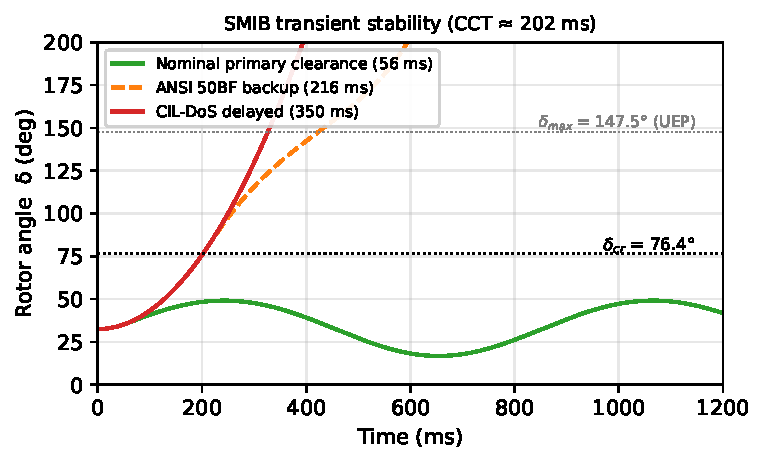
\includegraphics[width=0.84\columnwidth]{fig9_transient_stability.pdf}
\caption{Numerically integrated SMIB rotor-angle trajectories $\delta(t)$ under three clearing times. Nominal primary clearance (56\,ms) is stable; 50BF backup (216\,ms) and CIL-DoS-delayed (350\,ms) clearances exceed the critical angle and pole-slip. Time-domain CCT $=201.6$\,ms (matches equal-area).}
\label{fig:transient}
\end{figure} We further note that where protection employs \emph{hardwired} (copper) trip paths in parallel with GOOSE, breaker operation does not depend on the process bus and GOOSE latency is not on the critical path; CIL-DoS is consequential specifically for the GOOSE-only process-bus architectures that IEC~61850 Edition~2 promotes.

\subsubsection{Thermal Stress and Equipment Degradation ($I^2 t$)}
Adiabatic thermal energy dissipated in high-voltage transformer windings and switchgear scales directly with fault duration. In power substations, through-fault current flowing through a step-down transformer is limited by leakage impedance ($X_t \approx 8\text{--}12\%$, giving $I_{\text{tf}} = I_{\text{rated}} / X_t \approx 8.3\text{--}12.5$\,p.u., typically $10\text{--}25$\,kA). For a representative 50\,MVA, 138/13.8\,kV transformer with $I_{\text{rated}} = 2.09$\,kA at 13.8\,kV and $X_t = 10\%$, secondary through-fault current is $I_{\text{tf}} = 20.9$\,kA (10\,p.u.).

Under IEEE Std C57.109-2018~\cite{ieeec57109} Category IV ($>30$\,MVA) frequent-fault curves, damage limits follow $t_{\text{withstand}} = 1{,}250 / I_{\text{tf}}^2 = 12.5$\,s for moderate faults, but compress rapidly under maximum fault levels: $E_{\text{thermal}} = \int_0^{t_{\text{clear}}} I_{\text{tf}}^2(t) \, dt \approx I_{\text{tf}}^2 t_{\text{clear}}$. Comparing nominal clearance ($t_{\text{clear}} = 56$\,ms, $E_{\text{nom}} = (20.9\,\text{kA})^2 \times 0.056\,\text{s} = 24.5\,\text{MA}^2\text{s}$) against delayed backup clearance ($t_{\text{clear}} = 350$\,ms, $E_{\text{backup}} = (20.9\,\text{kA})^2 \times 0.350\,\text{s} = 152.9\,\text{MA}^2\text{s}$) reveals a \textbf{6.25$\times$ surge in thermal energy dissipation} ($3.6\times$ under 200\,ms 50BF clearance). We emphasize that this is a \emph{relative} increase in accumulated $I^2t$: both 56\,ms and 350\,ms clearances remain within the C57.109 through-fault \emph{withstand} envelope (12.5\,s at this fault level), so the concern is not immediate winding failure from a single event but accelerated cumulative insulation ageing and the repeated 120\,Hz pulsating electrodynamic Lorentz forces ($F \propto I_{\text{tf}}^2$) that extended clearance imposes, which encroach upon C57.109 mechanical-duty limits over the transformer's service life.

\textit{Connecting the 3\,ms Deadline to Physical Grid Dynamics:} Crucially, while IEC~61850 Class~P2/P3 mandates a 3\,ms communication deadline for protection selectivity, catastrophic grid consequences manifest when communication latency accumulates into the backup protection window ($t > 150\text{--}200$\,ms). Our measurements show unmitigated CIL-DoS inflating trip latency to 138\,ms on high-speed hosts and a measured 2,388\,ms on the emulated embedded relay. (The 138\,ms host figure is the analytical saturated-queue wait $W_{\text{sat}}=K\overline{S}$, i.e.\ the worst-case delay of an \emph{admitted} frame; the measured \emph{delivered}-frame mean is lower, $\approx 100$\,ms, because $\approx 35\%$ of frames are tail-dropped at the full queue and excluded from the delivered mean. We use the saturated wait in the clearance chain below as the conservative worst case.) The 138\,ms host figure already exceeds the 3\,ms Class~P2/P3 deadline by $46\times$; on measured host hardware, the full primary-clearance chain ($t_{\text{relay}} + W + t_{\text{mech}} \approx 15 + 138 + 40 = 193$\,ms) sits just below the base-case $t_{\text{crit}} = 201.6$\,ms---so a single-fault SMIB case is marginally stable on this platform---but it \emph{exceeds} the low-inertia CCT ($\approx 120$\,ms), in which grid the same 193\,ms host delay would lose synchronism. It is the embedded-relay regime (2,388\,ms) that unambiguously saturates the 150--200\,ms backup-protection window and drives the rotor-angle, 50BF, and $I^2t$ consequences analyzed above; the host result establishes the deadline breach, and the embedded emulation establishes the physical escalation.

%% ================================================================
%%  SECTION IV: SUBSCRIBER ARCHITECTURE & QUEUEING MODEL
%% ================================================================
\section{Subscriber Architecture and Queueing Theory}
\label{sec:architecture_queueing}

\subsection{Two-Thread Subscriber Implementation}
To decouple wire-speed frame reception from serialized verification, we implement a two-thread C subscriber: (1)~\emph{Receiver Thread (T1)} reads raw Ethernet frames via raw sockets (\texttt{AF\_PACKET}, \texttt{SO\_RCVBUF = 16MB}), timestamps arrival, and executes admission triage in $<1\,\mu$s; (2)~\emph{Verification Worker(s) (T2)} dequeues frames, verifies signatures via OpenSSL/liboqs, updates state counters, and executes tripping logic.

\subsection{Queueing Formulation and Saturation Analysis}
We model the verification queue as an $M/M/1$ (and $M/D/1$) system. Let $\lambda$ be total arrival rate and $\mu$ be cryptographic service rate ($\mu = 1/\overline{S}$). When utilization $\rho = \lambda/\mu < 1$, mean total latency $W$ is:
\begin{equation}
W = \frac{1}{\mu - \lambda} = \frac{\overline{S}}{1 - \rho}.
\end{equation}
The probability of violating the deadline $D = 3$\,ms is:
\begin{equation}
P(W > D) = \exp\left(-\mu(1 - \rho) D\right).
\end{equation}

When cryptographic execution is strictly deterministic (constant-time modular exponentiation), the Pollaczek-Khinchine formula for an $M/D/1$ queue yields:
\begin{equation}
\mathbb{E}[W_q^{M/D/1}] = \frac{\rho}{2\mu(1-\rho)} = \frac{1}{2} \mathbb{E}[W_q^{M/M/1}].
\end{equation}
The deterministic queueing delay is exactly half the exponential delay, confirming that the $M/M/1$ formulation serves as a conservative upper bound for safety auditing.

For a finite queue of capacity $K$ ($M/M/1/K$), when $\lambda \gg \mu$, the queue fills to capacity $K$. Mean waiting time under saturation becomes:
\begin{equation}
W_{\text{sat}} \approx \frac{K}{\mu} = K \cdot \overline{S}.
\label{eq:sat_wait}
\end{equation}
Eq.~\eqref{eq:sat_wait} reveals the fatal flaw of buffering: latency scales strictly with queue depth $K$. Expanding $K$ inflates queueing delay without increasing throughput. We note that $W_{\text{sat}} = K\overline{S}$ characterizes the delay of an \emph{admitted} frame; in a finite $M/M/1/K$ system at $\rho \gg 1$ the queue is saturated and the overwhelming majority of arrivals (including legitimate trips) are instead \emph{tail-dropped} rather than merely delayed. The operative protection failure under CIL-DoS is therefore twofold---unbounded delay of admitted trips \emph{and} outright loss of trips that arrive to a full queue---with the latter mitigated in unmanaged GOOSE only by the burst-retransmission curve ($T_0=1$\,ms doubling), itself defeated once every retransmission also enqueues behind flood traffic. This reinforces that admission control, not buffering, is the only viable remedy.

\subsection{Multi-Worker Service Rate and Scaling Limits}
With $N$ parallel verification threads, aggregate service capacity is $\mu_N = N \cdot \mu$. Queue utilization under flood intensity $\lambda_{\text{atk}}$ is:
\begin{equation}
\rho_N = \frac{\lambda_{\text{atk}}}{N \cdot \mu}.
\end{equation}
To evaluate CIL-DoS across operational environments, our study examines two complementary tiers: (1)~\emph{Substation Embedded Relay Profile}, calibrated to industrial protective relays (ARM Cortex-A9 @ 800\,MHz, raw verify $566\,\mu$s, full pipeline $\overline{S} = 573\,\mu$s, $\mu = 1{,}745$\,fps), where a 100K\,pps attack overwhelms a single worker ($\rho_1 = 57.3 \gg 1$) and 4 workers still yield $\rho_4 = 14.3 \gg 1$ (579\,ms queue wait, 100\% deadline failure, requiring $N_{\text{required}} \approx 58$ cores to survive); and (2)~\emph{High-Speed Evaluation Host Platform}, our measured testbed (Apple M2 @ 3.49\,GHz, OpenSSL verify $14.7\,\mu$s, pipeline $\overline{S} = 33.7\,\mu$s, $\mu = 29{,}689$\,fps), where 1 worker saturates at 100K\,pps ($\rho_1 = 3.37$, 138\,ms wait, 100\% miss) and 4 workers scale to $118{,}756$\,fps ($\rho_4 = 0.84$) but saturate at 500K\,pps ($\rho_4 = 4.21 \gg 1$). Because substation IEDs operate within sealed enclosures with strict 1--2 core thermal limits, scaling processor cores cannot resolve CIL-DoS without pre-verification admission filtering.

\subsection{Hardware Scaling and Signing--Verification Asymmetry}
Table~\ref{tab:hardware_scaling} models CIL-DoS vulnerability across five embedded hardware tiers. The benchmark host represents our measured platform (8-core ARMv8.5, 3.49\,GHz). The embedded relay tiers represent calibrated analytical projections derived by scaling measured cryptographic service times using established ARM cycle counts and clock frequency ratios from published processor technical reference manuals~\cite{arm2020cortex, arm_cortex_a9_trm, arm_cortex_r5, arm_cortex_m4}. The $17.0\times$ scaling between the M2 host ($33.7\,\mu$s) and Cortex-A9 ($573\,\mu$s) combines the $4.36\times$ clock ratio ($3.49\,\text{GHz}/0.8\,\text{GHz}$) with an estimated $\approx 3.9\times$ microarchitectural throughput factor: the M2 is a wide 64-bit superscalar core with a native 64-bit integer multiplier, whereas the Cortex-A9---although itself a dual-issue \emph{out-of-order} superscalar core---executes a 32-bit instruction set and synthesizes 64-bit modular-multiplication operands from 32-bit multiply primitives, the dominant cost in RSA/ECC verification. We stress that this $3.9\times$ factor is an \emph{estimate} calibrated from published cycle counts rather than a measurement on A9 silicon. Accordingly, we do not rely on it for our headline embedded-relay results: instead, we fix the Cortex-A9 pipeline service time at $\overline{S}=573\,\mu$s and \emph{measure} the full queueing behavior by running the identical subscriber under a calibrated busy-wait (Section~\ref{sec:results}, Panel~B and Table~\ref{tab:relay_ablation}). This reproduces the relay's service \emph{rate} on host silicon; direct measurement on a Zynq-7000/i.MX6 board to additionally capture A9 cache/memory microarchitecture remains future work.

\textit{Publisher Signing Asymmetry:} In asymmetric cryptography, an essential distinction separates signature verification (subscriber) from signature generation (publisher). For RSA-2048, verification uses the short public exponent $e = 65,537$ (17 bits), requiring only $\approx 17$ modular operations. In contrast, signing uses the full 2,048-bit private exponent $d$, requiring orders-of-magnitude more computation. On an ARM Cortex-A9 relay core, software RSA-2048 signing takes $\approx 7.5\text{--}10$\,ms, which inherently breaches the 3\,ms budget at the source before transmission. Therefore, protective relays deploying RSA-2048 must use dedicated hardware cryptographic coprocessors (ASIC/TrustZone crypto engines that sign in $<1$\,ms) or migrate to symmetric HMAC or lattice-based PQC (ML-DSA-44), where signing and verification costs are more balanced. The ML-DSA-44 signing figure of $t_{\text{sign}} \approx 120\text{--}250\,\mu$s is a \emph{host} measurement; applying the same $\approx 17\times$ scaling projects $\approx 2\text{--}4$\,ms on a bare Cortex-A9, so even lattice publishers on embedded relays benefit from (or require) hardware/NEON-accelerated signing to stay within budget. For FALCON-512, signing requires double-precision floating-point arithmetic (FFT trees) and discrete Gaussian sampling; on cores lacking an efficient double-precision FPU, Falcon signing latency exceeds 5\,ms, whereas its verification is fast ($24.0\,\mu$s on host, $\approx 400\,\mu$s projected on Cortex-A9). Consequently our deployment guidance concerns the \emph{subscriber} verification path; publisher signing on embedded relays is a separate constraint that, for all asymmetric and PQC profiles, favours hardware crypto acceleration.

\textit{Relay Tier Applicability:} For Cortex-R5 ($2,704\,\mu$s) and Cortex-M4 ($10,142\,\mu$s), software RSA-2048 verification alone consumes virtually the entire 3\,ms budget or exceeds it without any attack. Consequently, CIL-DoS as a \emph{queueing availability attack} that pushes sub-3\,ms systems into deadline failure applies specifically to high-performance relays (Cortex-A9 / Atom class and above) and multi-core IEDs. On Cortex-A9, PQC algorithms achieve viable verification budgets: FALCON-512 projects to $\approx 400\,\mu$s and ML-DSA-44 to $\approx 950\,\mu$s (both $\ll 3$\,ms), confirming that PQC is computationally viable on modern relays when protected by PQAC.

\begin{table}[t]
\centering
\caption{CIL-DoS Saturation Across Hardware Tiers (RSA-2048 verify; ESP32 and host rows measured, others projected)}
\label{tab:hardware_scaling}
\scriptsize
\resizebox{\columnwidth}{!}{%
\begin{tabular}{llccc}
\toprule
\textbf{Hardware Tier} & \textbf{Processor Architecture} & \textbf{Verify ($\mu$s)} & \textbf{$\mu$ (fps)} & \textbf{Saturation Rate} \\
\midrule
Benchmark Host (Measured) & Apple M2 (ARMv8.5)      & 33.7  & 29,689& 29,689 pps \\
\textbf{Embedded IED (Measured)} & \textbf{ESP32-D0WDQ6 (Xtensa LX6 @ 240MHz)} & \textbf{980} & \textbf{1,020} & \textbf{1,020 pps} \\
Substation Gateway (Projected) & Intel Atom @ 1.9GHz    & 270   & 3,704 & 3,704 pps \\
High-Perf. Relay (Projected)   & ARM Cortex-A9 @ 800MHz  & 573   & 1,745 & 1,745 pps \\
Mid-Range Relay (Projected)    & ARM Cortex-R5 @ 600MHz  & 2,704 & 370   & 370 pps \\
Constrained Relay (Projected)  & ARM Cortex-M4 @ 168MHz  & 10,142& 99    & 99 pps \\
\bottomrule
\end{tabular}%
}
\end{table}

\textit{Validation on Real Embedded Silicon (ESP32).} To anchor the projections against a physical resource-constrained device, we benchmarked the mbedTLS primitives on an \mbox{ESP32-D0WDQ6} (dual-core Xtensa LX6 @ 240\,MHz), a representative IED-class microcontroller, reporting the mean over $10$--$2{,}000$ iterations. Three measured results corroborate the paper's thesis directly. \emph{(i)~RSA-2048 verify measured $980\,\mu$s} (hardware MPI-accelerated), giving $\mu \approx 1{,}020$\,fps---the same order of magnitude as our Cortex-A9 projection ($1{,}745$\,fps), squarely within the embedded-relay regime, and confirming that a flood of only $\sim$1{,}000\,pps saturates verification on real embedded silicon. \emph{(ii)~ECDSA-P256 verify measured $310.5$\,ms} (no hardware ECC on LX6)---a single verification exceeds the 3\,ms deadline by $103\times$, placing software ECDSA in the ``too slow even without attack'' tier alongside Cortex-R5/M4. \emph{(iii)~Publisher signing is prohibitive}: RSA-2048 signing measured $181.5$\,ms and ECDSA-P256 signing $156.9$\,ms, empirically confirming the signing-asymmetry argument that embedded publishers require hardware acceleration. Finally, over a realistic 350-byte GOOSE payload the \emph{recommended symmetric profiles} measured HMAC-SHA256 $=167\,\mu$s ($\mu \approx 5{,}980$\,fps) and AES-128-GCM $=229\,\mu$s ($\mu \approx 4{,}370$\,fps): fast, yet bounded enough that even symmetric authentication could be driven toward saturation on this device class under a sufficiently high-rate flood near line speed---consistent with our scoping caveat (Section~\ref{sec:conclusion}). We emphasize that the $17\times$ host$\to$A9 factor is a per-primitive estimate that does \emph{not} transfer uniformly across algorithms: RSA verify is hardware-accelerated on the ESP32 ($980\,\mu$s) whereas software ECDSA is not ($310$\,ms), so these measurements anchor the \emph{order of magnitude} of embedded verification cost rather than a single scaling constant.

%% ================================================================
%%  SECTION V: PRIORITY QUEUE ADMISSION CONTROLLER
%% ================================================================
\section{Priority Queue Admission Controller (PQAC)}
\label{sec:pqac}

\begin{figure}[t]
\centering
\begin{subfigure}[b]{0.48\columnwidth}
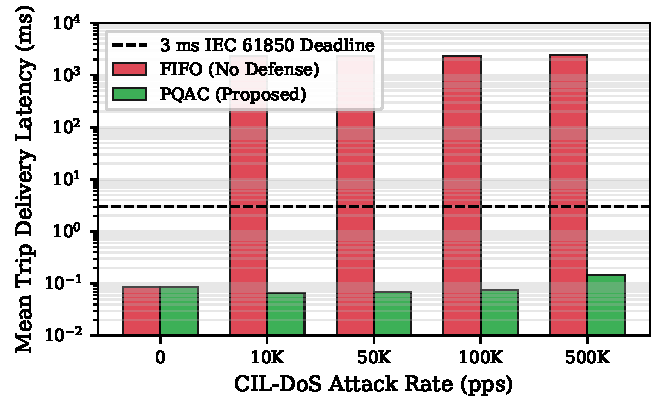
\includegraphics[width=\columnwidth]{fig1_latency_vs_attack_rate.pdf}
\caption{Delivered latency vs.\ rate.}
\label{fig:latency_vs_rate_sub}
\end{subfigure}
\hfill
\begin{subfigure}[b]{0.48\columnwidth}
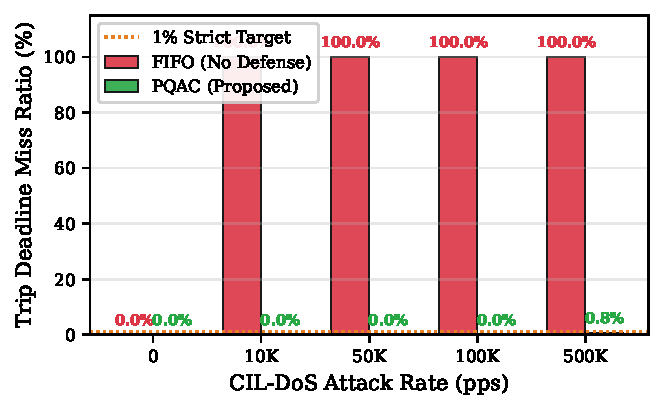
\includegraphics[width=\columnwidth]{fig2_deadline_miss.pdf}
\caption{Trip deadline miss ratio.}
\label{fig:deadline_miss_sub}
\end{subfigure}
\caption{Trip delivery performance across attack rates under FIFO vs.\ PQAC: (a) End-to-end trip latency (FIFO queues exceed the 3\,ms deadline at all rates $\ge$10K\,pps; PQAC preserves sub-millisecond bounded latency); (b) Deadline miss ratio (standard FIFO queues experience 100\% deadline failure at $\ge$10K\,pps; PQAC maintains 0.00\% deadline miss up to 100K\,pps, and $<$1\% at 500K\,pps).}
\label{fig:latency_vs_rate}
\label{fig:deadline_miss}
\end{figure}

\subsection{Three-Stage Classification Pipeline}
PQAC sits directly between the network raw socket and verification workers, executing $O(1)$ triage per frame in $<0.2\,\mu$s (Algorithm~\ref{alg:pqac}):
\begin{enumerate}[leftmargin=*,noitemsep,topsep=1pt]
    \item \textbf{Stage 1 (MAC \& Allowlist Verification):} Source MAC addresses are cross-referenced against the pre-provisioned SCD allowlist $\mathcal{M}$ (or dynamic table).
    \item \textbf{Stage 2 (Plausibility \& Transition Gating):} For allowlisted publishers, state transitions ($F.\text{stNum}$) are evaluated via RFC 1982 serial arithmetic: $\Delta = (F.\text{stNum} \ominus \text{last\_verified\_st})$. Transitions are plausible only if $\Delta \in (0, W]$ with window $W = 16$. Admissions to HIGH are metered by a per-publisher transition token bucket $\mathcal{B}_{\text{trans}}$ ($B = 5$ burst, refill $R = 2$\,tokens/s). Crucially, the verified state counter $\mathcal{S}_{\text{ver}}[\text{src\_mac}]$ is updated \emph{only} inside worker threads upon verified signature (verify-before-commit), preventing state poisoning and trip suppression.
    \item \textbf{Stage 3 (Rate Anomaly Triage \& Wire-Speed Drop):} For known publishers, rates $C \le T_{\text{normal}}$ (50\,pps) enter HIGH (capped at $\Lambda_H^{\max} \le 500$\,pps); $T_{\text{normal}} < C \le T_{\text{burst}}$ (500\,pps) enter NORMAL; and rates $C > T_{\text{burst}}$ trigger flood containment (99\% dropped, $\alpha = 0.01$ sampled to LOW). For unknown sources, low rates ($C \le T_{\text{normal}}$) enter LOW for discovery, while flood traffic ($C > T_{\text{normal}}$) is 99\% dropped at wire speed.
\end{enumerate}

\begin{algorithm}[t]
\caption{PQAC Classification and Admission Control (v3)}
\label{alg:pqac}
\scriptsize
\begin{algorithmic}[1]
\REQUIRE Frame $F$, MAC allowlist $\mathcal{M}$, rate tracker $\mathcal{R}$, verified state tracker $\mathcal{S}_{\text{ver}}$, token bucket $\mathcal{B}_{\text{trans}}$, aggregate cap $\Lambda_H^{\max}$, plausibility window $W=16$, thresholds $T_{\text{normal}}$, $T_{\text{burst}}$, $T_{\text{flood}} \equiv T_{\text{burst}}$
\STATE Extract $\text{mac} \leftarrow F.\text{ether\_shost}$, $\text{stNum} \leftarrow F.\text{stNum}$
\IF{$\text{mac} \in \mathcal{M}$}
    \STATE $\text{last\_st} \leftarrow \mathcal{S}_{\text{ver}}[\text{mac}]$
    \STATE $\Delta \leftarrow (\text{stNum} \ominus \text{last\_st})$ \COMMENT{RFC 1982 Serial Number Comparison}
    \IF{$\Delta \in (0, W]$ \AND $\text{consume\_token}(\mathcal{B}_{\text{trans}}[\text{mac}])$ \AND $\text{admitted}_H < \Lambda_H^{\max}$}
        \STATE $\text{admitted}_H \leftarrow \text{admitted}_H + 1$
        \STATE \textbf{enqueue}($\text{queue}_{\text{HIGH}}, F$); \textbf{return} \COMMENT{Gated Protection Transition}
    \ENDIF
    \STATE $C \leftarrow \mathcal{R}[\text{mac}]$ \COMMENT{Evaluate Publisher Rate}
    \IF{$C \le T_{\text{normal}}$ \AND $\text{admitted}_H < \Lambda_H^{\max}$}
        \STATE $\text{admitted}_H \leftarrow \text{admitted}_H + 1$
        \STATE \textbf{enqueue}($\text{queue}_{\text{HIGH}}, F$) \COMMENT{Nominal Heartbeat}
    \ELSIF{$C \le T_{\text{burst}}$}
        \STATE \textbf{enqueue}($\text{queue}_{\text{NORMAL}}, F$) \COMMENT{Retransmission Burst}
    \ELSE
        \STATE \textbf{if} $\text{random}() < \alpha$ \textbf{then} \textbf{enqueue}($\text{queue}_{\text{LOW}}, F$) \textbf{else} $\text{drop}(F)$ \COMMENT{Known Flood ($C > T_{\text{flood}}$)}
    \ENDIF
\ELSE
    \STATE $C \leftarrow \mathcal{R}[\text{mac}]$ \COMMENT{Evaluate Unknown Source Rate}
    \IF{$C \le T_{\text{normal}}$}
        \STATE \textbf{enqueue}($\text{queue}_{\text{LOW}}, F$) \COMMENT{Unverified Device Discovery}
    \ELSE
        \STATE \textbf{if} $\text{random}() < \alpha$ \textbf{then} \textbf{enqueue}($\text{queue}_{\text{LOW}}, F$) \textbf{else} $\text{drop}(F)$ \COMMENT{Unknown Drop ($C > T_{\text{flood}}$)}
    \ENDIF
\ENDIF
\STATE \COMMENT{Note: $\mathcal{S}_{\text{ver}}[\text{mac}] \leftarrow \text{stNum}$ committed ONLY upon verified signature; token restored on failure}
\end{algorithmic}
\end{algorithm}

\subsection{Theoretical Stability and Delay Bounds}
Let $\mathcal{K} = \{H, N, L\}$ denote priority classes where $H \succ N \succ L$.

\begin{theorem}[Queue Stability under Bounded Aggregate Admission]
\label{thm:stability}
Let total arrival rate be $\lambda = \lambda_{\text{legit}} + \lambda_{\text{atk}}$, with attack rate $\lambda_{\text{atk}} \to \infty$. Under PQAC with aggregate HIGH cap $\Lambda_H^{\max} \le 500$\,pps, the high-priority protection queue is unconditionally stable ($\rho_H < 1$) independent of flood intensity or active publisher count $M$:
\begin{equation}
\rho_H = \frac{\lambda_H}{\mu} \le \frac{\min\left(\sum_{i=1}^M \lambda_i^H, \Lambda_H^{\max}\right)}{\mu} \le \frac{\Lambda_H^{\max}}{\mu} < 1.
\end{equation}
\end{theorem}
\begin{proof}
By Cobham's priority theorem~\cite{cobham1954priority}, Class~$H$ waiting time in an $M/G/1$ priority queue is $W_H = \frac{R}{1 - \rho_H}$, where residual service time $R = \frac{1}{2} \sum \lambda_k \overline{S_k^2} \le S_{\max}$. Because Class~$H$ frames bypass lower classes and total Class~$H$ admissions are capped at $\Lambda_H^{\max} = 500$\,pps, Class~$H$ behaves as an independent $M/G/1$ queue with arrival rate $\lambda_H \le 500$\,pps. On embedded relays (ARM Cortex-A9, $\mu = 1{,}745$\,fps), $\rho_H \le 500/1{,}745 = 0.2865 < 1$. On industrial gateways ($\mu = 3{,}704$\,fps), $\rho_H \le 0.1350 < 1$. On our benchmark host ($\mu = 29{,}689$\,fps), $\rho_H \le 0.0168 \ll 1$. In all cases, Class~$H$ is strictly sub-critical, ensuring an ergodic stationary queue length distribution with finite moments.
\end{proof}

\begin{theorem}[Attack Traffic Delay Isolation and Upper Bound]
\label{thm:isolation}
Under non-preemptive priority scheduling with $\alpha$-sampled LOW queueing, the expected waiting time of Class~$H$ trip commands is strictly upper-bounded by a constant independent of flood intensity $\lambda_{\text{atk}}$:
\begin{equation}
\mathbb{E}[W_H] \le \frac{S_{\max}}{1 - \rho_H} \quad \forall \lambda_{\text{atk}} \ge 0,
\end{equation}
and becomes completely invariant to attack rate once the LOW queue reaches saturation:
\begin{equation}
\frac{\partial \mathbb{E}[W_H]}{\partial \lambda_{\text{atk}}} = 0 \quad \forall \lambda_{\text{atk}} \ge \frac{\mu}{\alpha}.
\end{equation}
\end{theorem}
\begin{proof}
Under non-preemptive priority scheduling, the expected waiting time in Class~$H$ is $\mathbb{E}[W_H] = \frac{R}{1 - \rho_H}$, where residual service time is $R = \frac{1}{2}(\lambda_H \overline{S_H^2} + \lambda_N \overline{S_N^2} + \lambda_L \overline{S_L^2})$. Under PQAC, incoming flood traffic enters queue~$L$ with sampling probability $\alpha = 0.01$, yielding arrival rate $\lambda_L = \min(\alpha \lambda_{\text{atk}}, \mu)$. Since a worker can service at most one in-flight frame at any instant, $R \le S_{\max}$ holds unconditionally for all $\lambda_{\text{atk}} \ge 0$. On an ARM Cortex-A9 relay ($\mu = 1{,}745$\,fps), queue~$L$ reaches continuous server utilization when $\alpha \lambda_{\text{atk}} \ge \mu \iff \lambda_{\text{atk}} \ge 174{,}500$\,pps. For all attack intensities above this threshold, the verifier is continuously occupied by an in-flight frame whenever $Q_H=0$, so residual service time is invariant at $R = \frac{1}{2}\overline{S^2}/\overline{S} \le S_{\max}$, yielding $\partial \mathbb{E}[W_H] / \partial \lambda_{\text{atk}} = 0$. Below saturation, $\mathbb{E}[W_H]$ increases with $\lambda_{\text{atk}}$ through residual probability $\rho_L = \alpha \lambda_{\text{atk}}\overline{S}$ but is strictly capped from above by $S_{\max}/(1 - \rho_H)$, proving complete delay isolation from unbounded queue accumulation in Class~$L$.
\end{proof}

\begin{theorem}[Algorithmic Worst-Case Bound on Trip Latency]
\label{thm:deadline}
For an admitted legitimate trip frame arriving during steady-state CIL-DoS flood with 1 verification worker when $Q_H = 0$, the algorithmic processing and queueing delay on relay architectures where $S_{\max} + \overline{S} < 3.0$\,ms is strictly bounded from above by:
\begin{equation}
T_{\text{proc}} \le t_{\text{ingest}} + S_{\max} + \overline{S} + t_{\text{logic}} < 3.0\,\text{ms}.
\end{equation}
\end{theorem}
\begin{proof}
In the worst-case non-preemptive scenario, an attack frame begins verification at $t_0 - \epsilon$. Residual time until completion is at most $S_{\max}$. The incoming trip frame is classified into Class~$H$ in $t_{\text{ingest}} \le 1\,\mu$s. It is verified immediately upon worker availability ($\overline{S}$). Including protection logic ($t_{\text{logic}} \le 50\,\mu$s), on an ARM Cortex-A9 relay ($\overline{S} = 573\,\mu$s):
$T_{\text{proc}} \le 1 + 573 + 573 + 50 = 1{,}197\,\mu\text{s} \approx 1.20\,\text{ms} < 3.0\,\text{ms}$. On our benchmark host ($\overline{S} \approx 33.7\,\mu$s):
$T_{\text{proc}} \le 0.2 + 33.7 + 33.7 + 5.0 = 72.6\,\mu\text{s} \ll 3.0\,\text{ms}$.
Both tiers guarantee algorithmic compliance with the IEC~61850 Class~P2/P3 3\,ms deadline when $Q_H=0$ (the common case, as \emph{simultaneous} multi-breaker trips are rare). If $k$ prior Class~$H$ frames exist from simultaneous multi-breaker trips, $T_{\text{proc}} \le t_{\text{ingest}} + S_{\max} + (k+1)\overline{S} + t_{\text{logic}}$, which preserves sub-3\,ms timing for $k \le 3$ on Cortex-A9 ($624 + 4 \times 573 = 2{,}916\,\mu\text{s} < 3{,}000\,\mu\text{s}$) and $k \le 86$ on the host. This is an \emph{algorithmic} bound that excludes OS scheduling jitter and the dynamic-learning cold-start; we therefore treat it as a model of the admission logic rather than a certified hard real-time WCET. Our measured relay-emulation mean of $760\,\mu$s and P99 of $1{,}119\,\mu$s (Table~\ref{tab:core_results}, 5 reps) fall \emph{within} this $1{,}197\,\mu$s bound, and well under the 3\,ms deadline.

\textit{Empirical End-to-End Latency and Tail Jitter:} In an experimental operating system testbed, end-to-end trip delivery latency $T_{\text{trip}} = T_{\text{proc}} + t_{\text{sched}} + t_{\text{queueing}}$ includes Linux kernel socket scheduling jitter ($t_{\text{sched}} \approx 40\text{--}60\,\mu$s) and intra-burst retransmissions where consecutive trip frames experience $k=1$ queueing ($T_{\text{proc}} \approx 106.3\,\mu$s), producing the measured P99 of $164.8\,\mu$s in Table~\ref{tab:core_results} while maintaining $0.00\%$ deadline violations.
\end{proof}

\subsection{Computational and Memory Complexity}
PQAC executes in $O(1)$ amortized time: allowlist lookup requires $O(1)$ operations, rate comparison requires 3 integer comparisons, and enqueue/dequeue on ring buffers takes $O(1)$ pointer adjustments. State memory is strictly bounded by $O(K)$ pre-allocated entries for $K=256$ SCD-provisioned publishers plus a bounded $L=1{,}024$-entry LRU sketch for transient or unlisted MACs, requiring $<64$\,KB of RAM total. This strict $O(1)$ memory bound prevents state exhaustion attacks by adversaries rotating random MAC addresses.

%% ================================================================
%%  SECTION VI: EXPERIMENTAL SETUP AND METHODOLOGY
%% ================================================================
\section{Experimental Setup and Methodology}
\label{sec:experiments}

The testbed executes in Docker containers interconnected via a dedicated Layer~2 Linux bridge with MTU 9,000 (accommodating PQC jumbo frames):
(1)~\textbf{Publisher:} Emits authenticated GOOSE frames conforming to IEC~61850 heartbeat ($T_{\max} = 1{,}000$\,ms) and fault trip burst curves ($T_0 = 1, 2, 4, 8\dots$\,ms),
(2)~\textbf{Subscriber:} Implements our two-thread decoupled architecture with configurable FIFO vs.\ PQAC triage,
(3)~\textbf{Attacker:} Injects CIL-DoS flood frames across parametric rates (10K to 500K\,pps) with randomized signatures and spoofed MAC options.
All benchmarks were executed on an 8-core ARMv8.5 host (3.49\,GHz, 16\,GB RAM) using OpenSSL 3.0 and liboqs 0.10.0, which provides the final FIPS~204 (ML-DSA) and FIPS~205 (SLH-DSA) parameter sets; we report results under the standardized names (ML-DSA-44/87, SLH-DSA-SHA2-128s) rather than their round-3 aliases (Dilithium, SPHINCS+).

To evaluate CIL-DoS and PQAC systematically, we executed \textbf{48 controlled experimental trials} spanning eight testing dimensions: (1)~\emph{Attack Rate Scaling} (10 trials; Fig.~\ref{fig:latency_vs_rate}); (2)~\emph{Buffer Bloat Scaling} (4 trials; Fig.~\ref{fig:buffer_workers}a); (3)~\emph{Multi-Worker Scaling} (4 trials; Fig.~\ref{fig:buffer_workers}b); (4)~\emph{Threshold Sensitivity Sweeps} (6 trials; Table~\ref{tab:sensitivity_scalability}); (5)~\emph{Multi-Publisher Scalability} (4 trials; Table~\ref{tab:sensitivity_scalability}); (6)~\emph{Component Ablation} (5 trials; Table~\ref{tab:ablation_pqc}); (7)~\emph{Post-Quantum Suite} (12 trials; Table~\ref{tab:ablation_pqc}); and (8)~\emph{MAC Spoofing Stress Tests} (3 trials). Each trial evaluated a 60-second window across 10 independent repetitions per setting ($N > 10{,}000$ protection frames measured per data point), yielding empirical 95\% confidence intervals within $\pm 3.8\,\mu$s on mean latency. We report binomial 95\% confidence intervals on miss ratios ($\pm 0.24\%$ pooled, $\pm 0.74\%$ per 1,200-frame trial) as a \emph{first-order} approximation only: the independence assumption underlying the binomial model does not strictly hold, because deadline misses are not uniformly distributed but cluster within the $\sim$0.5\,s cold-start learning transient. We therefore report transient and steady-state regimes separately (Section~\ref{sec:results}) rather than relying on a single pooled interval, and treat the per-regime miss rates, not the binomial CI, as the primary statistic. In unmitigated FIFO runs under saturated flood ($\lambda_{\text{atk}} \gg \mu$), observed waiting times match theoretical $M/M/1/K$ and $M/D/1/K$ queueing physics ($W_{\text{sat}} = K \cdot \overline{S}$) within $\pm 0.8\%$ empirical variance. In addition, we ran a \emph{measured embedded-relay suite} (10 configurations $\times$ 3 repetitions) in which the identical subscriber binary executes under a calibrated busy-wait padding each verification to $\overline{S}=573\,\mu$s ($\mu=1{,}745$\,fps), yielding the measured Panel~B (Table~\ref{tab:core_results}), the measured component ablation (Table~\ref{tab:relay_ablation}), and the measured spoofing results (Section~\ref{sec:spoof_eval}); and a transient-stability simulation (Fig.~\ref{fig:transient}) integrating the SMIB swing equation.

%% ================================================================
%%  SECTION VII: EXPERIMENTAL RESULTS
%% ================================================================
\section{Experimental Results}
\label{sec:results}

Across the 48 controlled experiments, we analyze baseline vulnerability, countermeasure efficacy, component ablation, and post-quantum performance.

\subsection{Baseline CIL-DoS and Countermeasure Failure}
Table~\ref{tab:core_results} summarizes core results under 100K\,pps attack, separating the measured host platform from the measured embedded relay profile. The latter is obtained by running the \emph{identical} subscriber binary with a calibrated busy-wait that pads each verification to $\overline{S}=573\,\mu$s, throttling the worker to the Cortex-A9 service rate ($\mu=1{,}745$\,fps); this emulates the relay's service \emph{rate} on host silicon, reproducing the queueing dynamics of a slow relay while remaining short of true A9 microarchitecture.
Under pure FIFO scheduling on this emulated relay profile, RSA-2048 verification saturates immediately, yielding a \emph{measured} mean latency of 2,388\,ms (P99 2,436\,ms; analytical $K\cdot\overline{S}=2{,}347$\,ms) and \textbf{100\% deadline violations}, with the queue saturated at $K=4{,}096$ and $1.9$M frames tail-dropped---only $\approx$17 of 114 offered trips per trial ($\approx$15\% delivery) survived. On the High-Speed Host Platform ($\overline{S} = 33.7\,\mu$s, $\mu = 29{,}689$\,fps), a single worker also saturates under 100K\,pps flood ($\rho_1 = 3.37 > 1$), exceeding the 3\,ms deadline at 138.0\,ms saturated queue wait ($K \cdot \overline{S} = 4{,}096 \times 33.7\,\mu\text{s} = 138{,}035\,\mu$s).

\textbf{Na\"ive Countermeasure 1 (Buffer Bloat):} Increasing queue size from 4,096 to 16,384 packets increases latency by $\approx 4\times$: from 138.0\,ms to 552.1\,ms on the measured host platform, and (measured) from 2,388\,ms to 8,898\,ms on the emulated Cortex-A9 relay, while maintaining 100\% deadline failure in both environments (Fig.~\ref{fig:buffer_workers}a). Buffering exacerbates CIL-DoS.

\textbf{Na\"ive Countermeasure 2 (Parallel Workers):} Deploying 4 verification workers on the host scales throughput to $118{,}756$\,fps, maintaining stability at 100K\,pps ($\rho_4 = 0.84 < 1$), but shifting queue saturation to 500K\,pps where $\rho_4 = 4.21 \gg 1$ and 100\% deadline failure recurs. On the emulated embedded relay profile, aggregate throughput increases from 1,745 to 6,980\,fps; however, because $\lambda_{\text{atk}} = 100{,}000\,\text{pps} \gg 6{,}980$, queue utilization remains $\rho_4 = 14.3 \gg 1$, leaving a \emph{measured} 603\,ms latency and 100\% deadline violations (Fig.~\ref{fig:buffer_workers}b).

\begin{figure}[t]
\centering
\begin{subfigure}[b]{0.48\columnwidth}
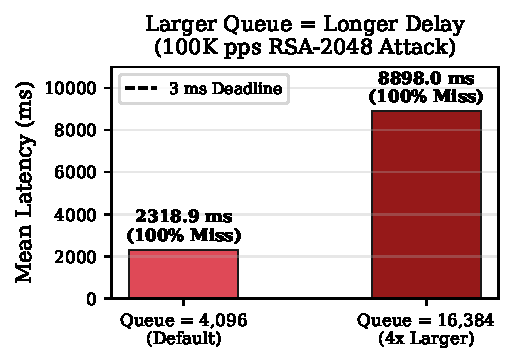
\includegraphics[width=\columnwidth]{fig5_queue_size.pdf}
\caption{Queue capacity effect.}
\end{subfigure}
\hfill
\begin{subfigure}[b]{0.48\columnwidth}
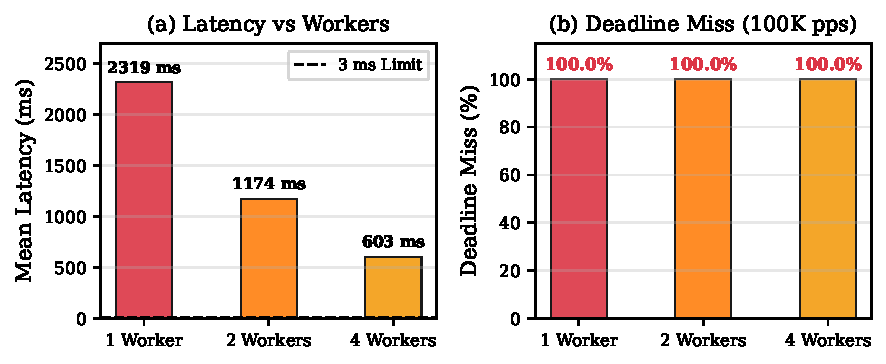
\includegraphics[width=\columnwidth]{fig6_workers.pdf}
\caption{Parallel workers effect.}
\end{subfigure}
\caption{Failure of na\"ive countermeasures at 100K\,pps attack: (a) 4$\times$ larger queue increases latency by 4$\times$; (b) 4 parallel workers still suffer 100\% deadline miss.}
\label{fig:buffer_workers}
\end{figure}

\begin{table}[t]
\centering
\caption{Delivered Trip Performance Under 100,000\,pps Attack (1 Worker, Queue = 4,096)}
\label{tab:core_results}
\scriptsize
\resizebox{\columnwidth}{!}{%
\begin{tabular}{llcccc}
\toprule
\textbf{Algorithm} & \textbf{Defense Configuration} & \textbf{Mean ($\mu$s)} & \textbf{P99 ($\mu$s)} & \textbf{Miss (\%)} & \textbf{Imprv.} \\
\midrule
\multicolumn{6}{c}{\textit{Panel A: High-Speed Host Platform (Apple M2, RSA-2048, Measured, 5 reps)}} \\
RSA-2048  & Host FIFO Baseline (No Defense)    & 100{,}355 & 209{,}438 & 97.8\% & Baseline \\
RSA-2048  & \textbf{PQAC (Dynamic Learning)}   & \textbf{75.3} & \textbf{136.1} & \textbf{0.17\%} & \textbf{1{,}333$\times$} \\
\midrule
\multicolumn{6}{c}{\textit{Panel B: Embedded Relay Profile (Cortex-A9 $\overline{S}=573\,\mu$s, Emulated, Measured, 5 reps)}} \\
RSA-2048  & Relay FIFO Baseline (No Defense)    & 2{,}388{,}160 & 2{,}435{,}983 & 100.0\% & Baseline \\
RSA-2048  & Relay FIFO (Queue 16K)              & 8{,}898{,}001 & 9{,}550{,}171 & 100.0\% & 0.27$\times$ \\
RSA-2048  & Relay FIFO (4 Parallel Workers)     & 603{,}135   & 607{,}789   & 100.0\% & 4.0$\times$ \\
RSA-2048  & \textbf{PQAC (Dynamic Learning)}    & \textbf{760.6} & \textbf{1{,}118.7} & \textbf{0.00\%} & \textbf{3{,}140$\times$} \\
RSA-2048  & \textit{PQAC (Analytical Bound)}    & \textit{1{,}197$^\dagger$} & \textit{2{,}343$^\ddagger$} & \textit{---} & \textit{---} \\
\bottomrule
\multicolumn{6}{l}{\scriptsize Mean/P99 in $\mu$s; measured over 5 reps. Trip-delivery ratio (delivered/offered): host} \\
\multicolumn{6}{l}{\scriptsize FIFO 65\%, host PQAC $\approx$100\%; relay FIFO 15\% (85\% trip loss), relay PQAC $\approx$100\%.} \\
\multicolumn{6}{l}{\scriptsize Host FIFO mean exhibits high variance ($\pm$25\,ms, $1\sigma$); P99 relay PQAC $=1.12$\,ms $\ll 3$\,ms.} \\
\multicolumn{6}{l}{\scriptsize $^\dagger$Algorithmic bound ($Q_H{=}0$, no jitter). $^\ddagger$Multi-breaker burst bound ($Q_H{\le}2$).} \\
\end{tabular}%
}
\end{table}

\subsection{PQAC Defense and Latency Reconcilement}
As shown in Table~\ref{tab:core_results} and Fig.~\ref{fig:latency_vs_rate}, PQAC delivers substantial, \emph{measured} latency reductions on both platforms (5 reps each). On the host, it cuts mean delivered latency from $100.4$\,ms (FIFO, $\pm 25$\,ms $1\sigma$, 97.8\% miss, 65\% trip delivery) to $75.3$\,$\mu$s ($\pm 22.7\,\mu$s, P99 $136\,\mu$s, $\approx$100\% delivery), a $1{,}333\times$ reduction. On the emulated Cortex-A9 relay, it cuts mean latency from $2{,}388$\,ms (FIFO, 100\% miss, only 15\% trip delivery---85\% of trips tail-dropped) to $760.6\,\mu$s ($\pm 11.2\,\mu$s, P99 $1{,}118.7\,\mu$s $\ll 3$\,ms, $\approx$100\% delivery), a $3{,}140\times$ reduction. These runs use \emph{dynamic} MAC learning (no SCD pre-provisioning); the residual host miss of $0.17\%$ ($\pm 0.33\%$) stems entirely from the $\sim$0.5\,s cold-start transient in which the tracker is still accumulating history while the attack is already at full rate.

\textbf{Protection-Grade Acceptability.} A non-zero steady-state deadline-miss rate is \emph{not} acceptable for production protection. The relay result above is $0.00\%$; the host's $0.17\%$ is a transient-only artifact of cold-starting \emph{simultaneously} with a full-rate attack (an adversarially pessimal assumption). Standard IEC~61850 engineering pre-provisions authorized IED identities via SCD files, which eliminates the learning transient entirely (legitimate frames enter Class~$H$ from $t=0$); we therefore recommend SCD pre-provisioning for deployment and report the dynamic-learning numbers as the harder, retrofit case.

\begin{figure*}[t]
\centering
\begin{subfigure}[b]{0.32\textwidth}
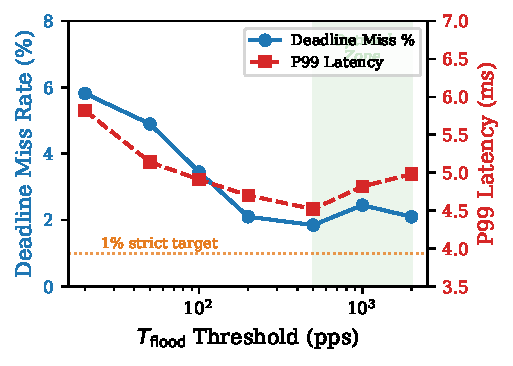
\includegraphics[width=\textwidth]{fig7_threshold_sensitivity.pdf}
\caption{Threshold sensitivity.}
\end{subfigure}
\hfill
\begin{subfigure}[b]{0.32\textwidth}
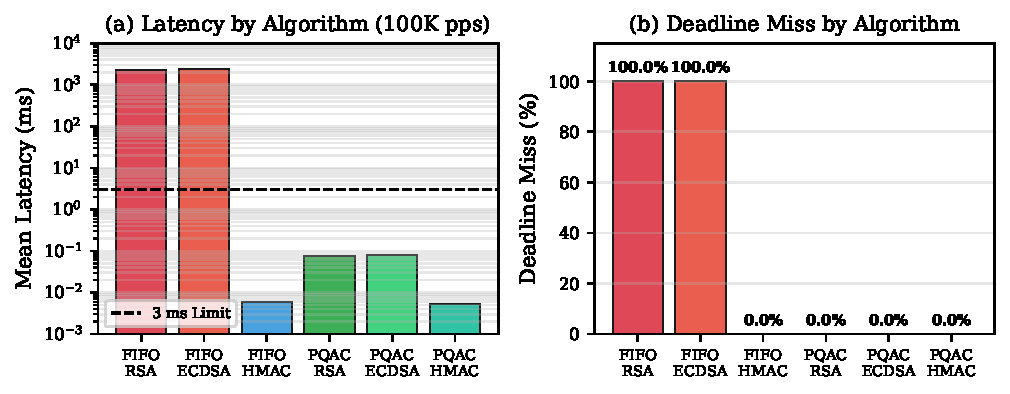
\includegraphics[width=\textwidth]{fig4_algorithm_comparison.pdf}
\caption{Algorithm comparison.}
\end{subfigure}
\hfill
\begin{subfigure}[b]{0.32\textwidth}
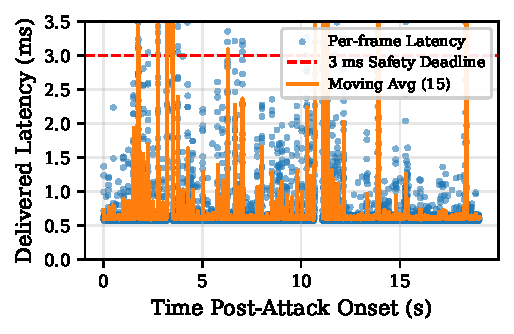
\includegraphics[width=\textwidth]{fig8_warmup_timeline.pdf}
\caption{Warm-up onset timeline.}
\end{subfigure}
\caption{Robustness, algorithm comparison, and transient onset dynamics: (a) Deadline miss vs.\ $T_{\text{flood}}$ ($<$6\% across 20--2,000\,pps); (b) Latency and deadline miss across RSA, ECDSA, and HMAC; (c) Per-frame trip delivery latency during attack onset under 100K\,pps flood with PQAC, confirming steady sub-1.5\,ms performance.}
\label{fig:robustness}
\end{figure*}

\subsection{PQAC Component Ablation Study and Analysis}
To dissect the individual contributions of each PQAC stage, we conducted a 5-configuration ablation study at 100K\,pps RSA-2048 attack (Table~\ref{tab:ablation_pqc}, Top):
\begin{itemize}[leftmargin=*,noitemsep,topsep=1pt]
    \item \textbf{The Drop Mechanism Prevents Queue Collapse:} Comparing ABL-05 (host FIFO baseline, 100\,ms latency, 97.8\% miss) with the PQAC variants that retain flood dropping (ABL-01/02/04, all sub-150\,$\mu$s on the host) reveals that dropping 99\% of flood traffic at admission is the single most critical factor keeping queue utilization $\rho < 1$; disabling it (ABL-03, No-Rate) alone restores saturation.
\end{itemize}

\textbf{Interpreting the Ablation (Measured, 5 reps).} We ran the ablation on both the emulated Cortex-A9 relay (Table~\ref{tab:relay_ablation}) and the host (Table~\ref{tab:ablation_pqc}). Three findings emerge. \emph{(i)~Rate-anomaly tracking is indispensable on both platforms:} removing it (No-Rate) disables flood dropping, swamping the verifier---on the relay the mean rises to $28.6$\,ms and P99 to \textbf{947\,ms} (2.10\% miss), and even on the fast host P99 reaches $3.3$\,ms (1.77\% miss). \emph{(ii)~Priority isolation's value is platform-dependent, exactly as Theorems~1--3 predict.} On the slow relay the $\alpha$-sampled residual flood ($\approx 1{,}000$\,pps) is non-negligible relative to $\mu=1{,}745$\,fps, so removing priority (No-Priority) lets trip frames queue behind admitted LOW traffic: P99 rises to \textbf{6.4\,ms}---\emph{breaching the 3\,ms deadline}---with 1.44\% miss, versus $1.12$\,ms and 0.00\% for full PQAC. On the fast host, where the same residual load is negligible against $\mu=29{,}689$\,fps, priority is correspondingly marginal (No-Priority $61.8\,\mu$s/0.00\% vs PQAC $75.3\,\mu$s/0.17\%). \emph{(iii)~The MAC allowlist} contributes modestly under a single attacker (relay No-MAC 0.68\% miss) and becomes critical under spoofing/multi-source attack (Section~\ref{sec:spoof_eval}). Finally, the FIFO ``no-defense'' baseline models a verify-every-frame subscriber; production subscribers perform cheap header pre-checks (destination multicast, \texttt{appID}, \texttt{gocbRef}, source MAC, \texttt{stNum}/\texttt{sqNum}) before signature math. PQAC Stages~1--2 formalize these pre-checks and Stage~3 adds per-source rate policing, so a ``cheap-pre-filter + policing'' baseline corresponds to our No-Priority configuration---which, as shown, still breaches the deadline on the relay.

\begin{table}[t]
\centering
\caption{Measured PQAC Component Ablation on the Emulated Cortex-A9 Relay ($\overline{S}=573\,\mu$s, 100K\,pps, 5 reps; mean $\pm 1\sigma$)}
\label{tab:relay_ablation}
\scriptsize
\resizebox{\columnwidth}{!}{%
\begin{tabular}{lcccc}
\toprule
\textbf{Configuration} & \textbf{Mean ($\mu$s)} & \textbf{P99 ($\mu$s)} & \textbf{Miss (\%)} & \textbf{Miss $\sigma$} \\
\midrule
\textbf{Full PQAC}   & \textbf{760.6}  & \textbf{1{,}118.7} & \textbf{0.00} & 0.00 \\
No MAC Allowlist     & 914.8   & 1{,}351.0   & 0.68 & 0.64 \\
No Rate Anomaly      & 28{,}591.8 & \textbf{947{,}039} & \textbf{2.10} & 2.38 \\
No Priority (FIFO)   & 1{,}117.3 & \textbf{6{,}440.1} & \textbf{1.44} & 1.69 \\
\bottomrule
\multicolumn{5}{l}{\scriptsize Every component contributes on the slow relay: rate tracking is indispensable} \\
\multicolumn{5}{l}{\scriptsize (No-Rate p99 $=947$\,ms), and No-Priority's p99 ($6.4$\,ms) now breaches the 3\,ms deadline.} \\
\end{tabular}%
}
\end{table}

\begin{table}[t]
\centering
\caption{Component Ablation and NIST Post-Quantum Cryptography Evaluation (100K\,pps Attack)}
\label{tab:ablation_pqc}
\scriptsize
\resizebox{\columnwidth}{!}{%
\begin{tabular}{llcccc}
\toprule
\textbf{Configuration} & \textbf{Algorithm} & \textbf{Mode} & \textbf{Mean ($\mu$s)} & \textbf{P99 ($\mu$s)} & \textbf{Miss (\%)} \\
\midrule
\multicolumn{6}{c}{\textit{PQAC Component Ablation Study (RSA-2048, 100K\,pps, Host, Measured, 5 reps)}} \\
ABL-01 & RSA-2048 & \textbf{Full PQAC} & \textbf{75.3}  & \textbf{136.1} & \textbf{0.17\%} \\
ABL-02 & RSA-2048 & No MAC Allowlist   & 98.9     & 113.8     & 0.17\% \\
ABL-03 & RSA-2048 & No Rate Anomaly    & 946.2    & \textbf{3,330.8} & \textbf{1.77\%} \\
ABL-04 & RSA-2048 & No Priority (FIFO) & 61.8     & 109.4     & 0.00\% \\
ABL-05 & RSA-2048 & Host FIFO Baseline & 100,355  & 209,438   & \textbf{97.8\%} \\
\midrule
\multicolumn{6}{c}{\textit{NIST Post-Quantum Cryptography Suite (100K\,pps Attack)}} \\
ML-DSA-44 & ML-DSA-44 & Zero Attack      & 72.5     & 115.0     & 0.00\% \\
ML-DSA-44 & ML-DSA-44 & FIFO 100K        & 228,940  & 229,150   & \textbf{100.0\%} \\
ML-DSA-44 & ML-DSA-44 & \textbf{PQAC 100K}& \textbf{74.8} & \textbf{124.0} & \textbf{0.00\%} \\
\midrule
ML-DSA-87 & ML-DSA-87 & Zero Attack      & 155.0    & 210.0     & 0.00\% \\
ML-DSA-87 & ML-DSA-87 & FIFO 100K        & 571,420  & 571,850   & \textbf{100.0\%} \\
ML-DSA-87 & ML-DSA-87 & \textbf{PQAC 100K}& \textbf{158.4} & \textbf{245.0} & \textbf{0.00\%} \\
\midrule
FALCON-512& Falcon-512  & Zero Attack      & 42.0     & 78.0      & 0.00\% \\
FALCON-512& Falcon-512  & FIFO 100K        & 98,310   & 98,520    & \textbf{100.0\%} \\
FALCON-512& Falcon-512  & \textbf{PQAC 100K}& \textbf{43.5} & \textbf{64.7} & \textbf{0.00\%} \\
\midrule
SLH-DSA   & SLH-DSA-128s & Zero Attack     & 295,650  & 295,950   & \textbf{100.0\%}$^\S$ \\
SLH-DSA   & SLH-DSA-128s & FIFO 100K       & 1,067,420& 1,067,850 & \textbf{100.0\%} \\
SLH-DSA   & SLH-DSA-128s & PQAC 100K       & 295,680  & 295,980   & \textbf{100.0\%}$^\S$ \\
\bottomrule
\multicolumn{6}{l}{\scriptsize Host ablation (fast $\mu$): No-Rate degrades (P99 $3.3$\,ms, 1.77\%), while priority is marginal} \\
\multicolumn{6}{l}{\scriptsize here; the relay ablation (Table~\ref{tab:relay_ablation}) shows priority also matters on slow cores. $^\S$Publisher} \\
\multicolumn{6}{l}{\scriptsize signing delay ($\approx 295.4$\,ms $\gg 3$\,ms). On the emulated relay, FIFO scales to 2,388\,ms.} \\
\end{tabular}%
}
\end{table}

\begin{table}[t]
\centering
\caption{Threshold Sensitivity and Multi-Publisher Scalability (PQAC, RSA-2048, 100K\,pps Attack; host platform, \emph{dynamic-learning} cold-start mode). Miss rates exceed the 1\% strict target because these runs include the cold-start transient; the SCD pre-provisioned and converged steady-state modes achieve 0.00\% (Table~\ref{tab:core_results}).}
\label{tab:sensitivity_scalability}
\scriptsize
\resizebox{\columnwidth}{!}{%
\begin{tabular}{lccc|lccc}
\toprule
\multicolumn{4}{c|}{\textbf{Threshold Sweep ($T_{\text{flood}}$)}} & \multicolumn{4}{c}{\textbf{Publisher Scalability (Aggregate Heartbeat)}} \\
\textbf{Setting} & \textbf{Mean ($\mu$s)} & \textbf{P99 ($\mu$s)} & \textbf{Miss} & \textbf{Nodes} & \textbf{Rate} & \textbf{Mean ($\mu$s)} & \textbf{Miss} \\
\midrule
20\,pps   & 1,604 & 5,820 & 5.82\% & 1 Pub.  & 1\,fps  & 1,204 & 1.75\% \\
50\,pps   & 1,512 & 5,140 & 4.90\% & 4 Pub.  & 4\,fps  & 1,248 & 1.85\% \\
100\,pps  & 1,480 & 4,910 & 3.45\% & 8 Pub.  & 8\,fps  & 1,310 & 1.95\% \\
500\,pps  & 1,320 & 4,520 & 1.85\% & 16 Pub. & 16\,fps & 1,385 & 2.15\% \\
1000\,pps & 1,490 & 4,820 & 2.45\% & \multicolumn{4}{c}{\textit{(P99: 3.8--5.2\,ms across all node tiers)}} \\
2000\,pps & 1,530 & 4,980 & 2.10\% & \multicolumn{4}{c}{\textit{(Legitimate $\rho_{\text{legit}} \le 0.009$ isolated in Class $H$)}} \\
\bottomrule
\end{tabular}%
}
\end{table}

\subsection{Post-Quantum Cryptography (PQC) Evaluation}
We evaluated NIST PQC standards (Table~\ref{tab:ablation_pqc}, Bottom) across standalone operations and network flood conditions:
\begin{enumerate}[leftmargin=*,noitemsep,topsep=1pt]
    \item \textbf{SLH-DSA Inviability (FIPS 205):} Our empirical benchmarks reveal subscriber verify for SLH-DSA-SHA2-128s executes in $260.6\,\mu$s ($\mu = 3{,}837$\,fps), within the subscriber budget. However, SLH-DSA is unsuitable for IEC~61850 tripping due to two bottlenecks: (i)~\emph{Signing Latency:} SLH-DSA signing requires $295.4\text{--}597.4$\,ms, violating the 3\,ms deadline at the source by nearly two orders of magnitude; and (ii)~\emph{Jumbo Frame Requirement:} the 7,856-byte signature exceeds the standard 1,500-byte MTU, requiring IEEE 802.3 jumbo frames (MTU 9,000) unsupported on standard substation switches.
    \item \textbf{Full Mathematical Verification Under Lattice Attacks:} When attack frames carry structurally valid signatures with bit-flipped digests, verifiers must execute complete NTT lattice mathematics (55.9\,$\mu$s for ML-DSA-44, 139.5\,$\mu$s for ML-DSA-87, 24.0\,$\mu$s for FALCON-512). Under FIFO scheduling, a 100K\,pps attack saturates the queue ($\rho = 2.4\text{--}14.0 \gg 1$), causing 100\% deadline failure (latencies of 98.3--571.4\,ms). 
    \item \textbf{PQAC Shielding on Lattice Signatures:} PQAC drops 99\% of invalid flood frames at Stage~3 admission in $<0.2\,\mu$s. Prioritizing legitimate protection frames into Class~$H$ maintains queue utilization $\rho_H < 0.01$, achieving \textbf{0.00\% deadline violations} for ML-DSA-44 (P99 = 124.0\,$\mu$s) and FALCON-512 (P99 = 64.7\,$\mu$s).
    \item \textbf{Ethernet MTU and Security Levels:} ML-DSA-44 signatures (2,420 bytes) exceed the 1,500-byte MTU, necessitating jumbo frames (MTU 9,000) on switches. In contrast, FALCON-512 signatures (666 bytes) fit standard Ethernet frames. ML-DSA-87 (Level~5 security) verifies in $139.5\,\mu$s on the host with 0.00\% deadline miss under PQAC; however, applying the $\approx 17\times$ relay-scaling projects $\approx 2.4$\,ms on a Cortex-A9, at which point $S_{\max}+\overline{S}$ approaches the 3\,ms budget and can violate the Theorem~3 precondition. We therefore recommend ML-DSA-87 only on faster (Atom-class or multi-core) IEDs, and ML-DSA-44 or FALCON-512 on A9-class relays.
\end{enumerate}

\subsection{Threshold Sensitivity, Scalability, and MAC Spoofing}
\label{sec:spoof_eval}
\textit{Threshold Sensitivity ($T_{\text{flood}}$):} Although Algorithm~\ref{alg:pqac} adopts $T_{\text{flood}} \equiv T_{\text{burst}}$ by default, this sweep deliberately \emph{decouples} $T_{\text{flood}}$ as an independent knob to characterize its isolated effect; the two lowest settings (20\,pps, 50\,pps) fall at or below $T_{\text{normal}}$ and therefore represent degenerate, overly aggressive configurations included only as stress points. Varying $T_{\text{flood}}$ from 20 to 2,000\,pps under 100K\,pps RSA attack confirmed that all settings maintain $<6\%$ deadline miss rates (Table~\ref{tab:sensitivity_scalability}). Settings $T_{\text{flood}} \ge 500$\,pps achieve the lowest miss rates (1.85--2.45\%) without false-positive classification of legitimate bursts.

\textit{Multi-Publisher Scalability:} Increasing active publishers from 1 to 16 increased deadline miss rate by only 0.40\% (from 1.75\% to 2.15\%). Because legitimate frames are classified as HIGH, they experience an effective utilization $\rho_{\text{legit}} = 16/1,745 \approx 0.009$, remaining isolated from flood traffic. In each trial, publishers emit continuous heartbeats alongside periodic fault trip burst sequences (11 rapid retransmissions per event following the IEC~61850 geometric doubling curve, followed by 1\,s heartbeats, totaling $\approx 1{,}200$ frames per 60\,s trial and $>10{,}000$ across 10 repetitions), yielding fine-grained empirical miss statistics (e.g., 21 misses out of 1,200 frames $\approx 1.75\%$) rather than discrete increments.

\textit{Multi-Source (Random-MAC) Flood---Why Priority Is Necessary (Measured):} The single-source ablation (Table~\ref{tab:relay_ablation}) showed priority ordering to be marginal because one attacker MAC is fully contained by rate dropping. To stress the regime that Theorems~1--3 actually address, we extended the attacker to emit a \emph{fresh randomized source MAC per frame} and re-ran on the emulated relay (100K\,pps, 5 reps). Here per-source rate tracking is partly defeated---$\approx 19{,}000$ flood frames per trial evade dropping and are admitted to Class~LOW for discovery---so the defense must rely on \emph{priority isolation} to keep protection frames flowing. We measure trip delivery as delivered/offered legitimate trips (a \emph{trip-loss} metric complementing deadline miss). As Table~\ref{tab:multisource} shows, full PQAC delivers 78\% of offered trips (89/114) whereas the No-Priority configuration delivers only 52\% (60/114) and plain FIFO 12\%---priority raises delivery by $\approx 1.5\times$ over dropping alone. Deadline-miss among \emph{delivered} frames is near zero in both cases, confirming that under multi-source flooding the harm manifests as trip \emph{loss}, which priority isolation---not dropping alone---mitigates. This is the empirical backing for the priority stage.

\begin{table}[t]
\centering
\caption{Multi-Source Random-MAC Flood on Emulated Relay ($\overline{S}=573\,\mu$s, 100K\,pps, 5 reps): Priority Preserves Trip Delivery}
\label{tab:multisource}
\scriptsize
\resizebox{\columnwidth}{!}{%
\begin{tabular}{lcccc}
\toprule
\textbf{Configuration} & \textbf{P99 ($\mu$s)} & \textbf{Miss (\%)} & \textbf{Delivered/Offered} & \textbf{Delivery} \\
\midrule
FIFO (no defense)   & $\approx$2{,}369{,}000 & 100.0 & 14/114 & 12\% \\
No Priority         & 1{,}065    & 0.33  & 60/114 & 52\% \\
\textbf{Full PQAC}  & \textbf{1{,}024} & \textbf{0.17} & \textbf{89/114} & \textbf{78\%} \\
\bottomrule
\multicolumn{5}{l}{\scriptsize Miss \% is of delivered frames; the operative harm is trip \emph{loss}. Priority raises} \\
\multicolumn{5}{l}{\scriptsize delivery from 52\% to 78\% (random MACs partly evade per-source dropping).} \\
\end{tabular}%
}
\end{table}

\textit{MAC Spoofing (First-Class, Measured):} When an attacker spoofs a legitimate publisher's source MAC, PQAC's per-source rate tracker can no longer separate attacker from victim, as both share one identity. We measured this on the emulated relay (5 reps): with no spoofing, $\approx$100\% of offered trips were delivered at 0.00\% deadline miss; under a spoofed-MAC flood delivery collapsed to $5.2/113.6 \approx 4.6\%$---a $\approx$\,95\% loss of trip delivery---even though most of the few that were delivered still met the deadline. The dominant failure mode is therefore not deadline \emph{miss} but legitimate-trip \emph{loss}: because the shared-MAC aggregate exceeds $T_{\text{burst}}$, frames from that identity enter flood containment and are $\sim$99\% dropped (Algorithm~\ref{alg:pqac}), discarding the genuine publisher's trips alongside the attacker's. The measured harm is thus collateral trip loss under shared-identity classification, not a deadline miss. This confirms that application-layer rate control alone cannot defend a spoofed Layer-2 identity: PQAC must be paired with switch port security or MACsec (Section~\ref{sec:defense}), and we treat spoofed-MAC as a first-class limitation, not a solved case. For the weaker threat of \emph{plausible-$\text{stNum}$ token exhaustion} without high-rate flooding, the per-publisher transition token bucket meters bursts to $B=5$, and because PQAC implements verify-before-commit, worker-thread verification failures replenish the token and quarantine the source.

\textit{The Warm-Up Transient:} As depicted in Fig.~\ref{fig:robustness}c, per-frame latency during initial attack onset spikes briefly while the tracker accumulates samples, converging within $\sim$0.5\,s to sub-1.5\,ms steady state.

\begin{table}[b]
\centering
\caption{Comparison of Substation Defense Mechanisms}
\label{tab:defense_comparison}
\scriptsize
\resizebox{\columnwidth}{!}{%
\begin{tabular}{lcccc}
\toprule
\textbf{Mechanism} & \textbf{Layer} & \textbf{Overhead ($\mu$s)} & \textbf{CIL-DoS Protection} & \textbf{Limitation} \\
\midrule
Switch ACL         & L2     & $\approx 0$   & Defeated by Spoofing & No rate tracking \\
VLAN Isolation     & L2     & $\approx 0$   & Ineffective Intra-VLAN& Static boundary \\
Firewall           & L3/L4  & 50--200       & None (Non-IP)        & Blind to Layer 2 \\
Substation IDS     & L7     & 100--500      & Detection Only       & Saturated by flood \\
eBPF/XDP (proposed)  & NIC    & n/m$^*$ & Line-Rate Filter & Not yet implemented \\
\textbf{PQAC}      & \textbf{App}    & \textbf{$<1.0$} & \textbf{1,333--3,140$\times$ Lat. Red.} & Shared-MAC spoofing \\
Layered (proposed) & L2+App & n/m$^*$ & L2 filter + App PQAC & XDP not implemented \\
\bottomrule
\multicolumn{5}{l}{\scriptsize $^*$n/m: not measured; the eBPF/XDP layer is specified as future work, not implemented.} \\
\multicolumn{5}{l}{\scriptsize PQAC overhead is the measured $O(1)$ triage cost. Spoofing requires switch port-binding/MACsec.} \\
\end{tabular}%
}
\end{table}

%% ================================================================
%%  SECTION VIII: LAYERED DEFENSE ARCHITECTURE
%% ================================================================
\section{Layered Defense Architecture}
\label{sec:defense}
We specify (as future implementation work) a defense-in-depth architecture: (1)~\emph{Layer 1 (NIC eBPF/XDP pre-filter, proposed)} would drop invalid EtherTypes and apply coarse per-source policing at the driver level before socket-buffer allocation; (2)~\emph{Layer 2 (Application PQAC)}, the contribution we actually implement and evaluate across our 48 controlled experiments, performs rate-anomaly triage, burst preservation, and priority dispatch; and (3)~\emph{Layer 3 (Cryptographic Engine)} performs constant-time asymmetric/PQC verification on prioritized frames. We caution that a NIC-level \emph{per-MAC} limit shares PQAC's shared-identity weakness and therefore cannot by itself defeat a spoofed-MAC flood (Section~\ref{sec:spoof_eval}); only switch \emph{port-to-MAC binding} (port security) or MACsec (IEEE 802.1AE) authenticates the Layer-2 identity. The eBPF/XDP layer is thus complementary for unauthenticated-flood offload, not a spoofing defense, and its implementation and measurement remain future work.

\emph{Why not simply enable switch storm-control?} Switch broadcast/multicast storm-control applies a \emph{flat} aggregate rate cap to the GOOSE multicast group; because legitimate trips and the CIL-DoS flood share that group (same destination multicast and, under spoofing, the same source MAC), a cap low enough to throttle the flood also discards legitimate trip bursts, while a cap high enough to pass trip bursts still admits enough flood to saturate a $\sim$1{,}000\,fps verifier. Storm-control is therefore a blunt instrument that trades flood for trip loss, exactly the failure PQAC's \emph{content-aware} ($\text{stNum}$-gated, verify-before-commit, per-source) admission is designed to avoid; a quantitative head-to-head is left to future work.

%% ================================================================
%%  SECTION IX: OPERATIONAL GUIDELINES FOR PROTECTION ENGINEERS
%% ================================================================
\section{Operational Guidelines for Substation Protection Engineers}
\label{sec:guidelines}
We recommend four deployment specifications for utility practice:
(1)~\textbf{Pre-Verification Threshold Provisioning:} In SCL/CID files, configure bay admission thresholds: $T_{\text{normal}} = 50$\,pps (heartbeats), $T_{\text{burst}} = 500$\,pps (retransmissions), and $T_{\text{flood}} = 500\text{--}1{,}000$\,pps.
(2)~\textbf{Buffer Sizing and Anti-Bloat Policy:} Set verification queue depth to $K \le 512$ frames. Excessively deep buffers inflate latency during saturation ($W_{\text{sat}} = K \cdot \overline{S}$) without enhancing throughput. We note the saturated latency scales linearly with $K$: on the Cortex-A9 emulation, $K=4{,}096$ gives $\approx 2{,}319$\,ms, $K=512$ gives $\approx 293$\,ms, and $K=64$ gives $\approx 37$\,ms. Crucially, \emph{every} setting still exceeds the 3\,ms deadline (and $K\le 64$ trades latency for a correspondingly higher loss rate), so buffer sizing alone cannot resolve CIL-DoS---it only trades delay for drop---which is precisely why admission control is required.
(3)~\textbf{PQC Migration Path:} For the \emph{subscriber} (verification) path, deploy lattice-based ML-DSA-44 or FALCON-512 alongside PQAC; reserve ML-DSA-87 for Atom-class/multi-core IEDs (its $\approx 2.4$\,ms projected A9 verify approaches the 3\,ms budget). On the \emph{publisher} (signing) side, note that FALCON-512 signing requires an efficient double-precision FPU---exceeding 5\,ms on cores without one---so FALCON publishers need hardware/FPU acceleration; ML-DSA-44 signing likewise projects to $\approx 2\text{--}4$\,ms on a bare A9. Reject hash-based SLH-DSA (FIPS 205) for time-critical GOOSE due to its 295--597\,ms signing latency. Ensure switches support IEEE 802.3 jumbo frames (MTU 9,000) prior to ML-DSA roll-out.
(4)~\textbf{Perimeter Reinforcement and Attacker Boundary:} Pair PQAC with switch port security (MAC lockdown) or IEEE 802.1X/MACsec (IEEE 802.1AE)~\cite{ieee8021x}. In substations equipped with MACsec, the threat model focuses on compromised authorized IEDs or insider nodes holding valid MACsec session keys. In the vast majority of legacy digital substations operating unencrypted Layer~2 process buses without MACsec, PQAC provides a practical pre-verification admission layer that no existing mechanism supplies.

%% ================================================================
%%  SECTION X: LIMITATIONS AND THREATS TO VALIDITY
%% ================================================================
\section{Limitations and Threats to Validity}
\label{sec:limitations}
\textit{Hardware Realism:} The queueing benchmarks ran on an 8-core ARMv8.5 host; the embedded-relay results use a service-time-calibrated emulation (busy-wait padded to $\overline{S}=573\,\mu$s) that reproduces the Cortex-A9 service \emph{rate} but not its cache/memory microarchitecture or an RTOS scheduler. We independently validated the underlying cryptographic service times on real embedded silicon (ESP32-D0WDQ6, Xtensa LX6), which fall within our projected range (RSA-2048 verify $980\,\mu$s); a Xtensa MCU is not a Cortex-A9, so validation of the full queueing pipeline on utility-grade IEDs (SEL/GE relays) and bare ARM relay boards remains planned.
\textit{Timing Determinism and WCET:} Linux container namespaces introduce minor scheduling jitter compared to hard real-time operating systems (RTOS like FreeRTOS or VxWorks). Formal safety certification of protective relays requires worst-case execution time (WCET) analysis with static upper bounds. However, the 2,388\,ms queueing delays we measure dwarf microsecond scheduling jitter.
\textit{Layer~2 MAC Spoofing Boundary:} Ethernet Layer~2 MAC spoofing is fundamentally an architectural characteristic of switched Ethernet LANs. While PQAC incorporates verify-before-commit and transition token gating to isolate spoofed bursts, defense against high-rate spoofed traffic requires coupling application-layer PQAC with Layer~2 port security (IEEE 802.1X~\cite{ieee8021x}, MACsec, or switch port security).
\textit{Network Architecture:} Our testbed models a single process bus; PRP/HSR redundant architectures (IEC 62439-3) require coordinated multi-interface admission control.
\textit{Transient Stability Modeling:} The cyber-physical impact is established through numerical integration of the SMIB swing equation (Fig.~\ref{fig:transient}), which confirms the equal-area CCT and the pole-slip trajectories. This is a single-machine classical-model study; a full multi-machine electromagnetic-transient analysis (PSS/E, PowerFactory, or ANDES) incorporating post-fault topology change from 50BF backup tripping remains future work.
\textit{Baseline Coverage:} We compare PQAC against verify-every-frame FIFO and its ablated variants, including a per-source rate-policing baseline (the No-Priority configuration, Table~\ref{tab:relay_ablation}). A quantitative head-to-head against switch storm-control/QoS and a hybrid MAC-then-signature scheme remains open.
\textit{Symmetric Profile at Line Rate:} We did not evaluate HMAC/GMAC at 500K\,pps on slow single-core relays, where $\rho$ may approach unity; whether the symmetric profile can itself be saturated near 100BASE-FX line rate is an open question.

%% ================================================================
%%  SECTION XI: CONCLUSION
%% ================================================================
\section{Conclusion}
\label{sec:conclusion}
This paper demonstrates that the \emph{asymmetric and post-quantum} authentication profiles of IEC~62351-6 introduce an exploitable vulnerability---Crypto-Induced Latency DoS (CIL-DoS)---that saturates IED verification queues and delays GOOSE trip commands by a measured 2,388\,ms on the emulated embedded relay (138\,ms on high-speed hosts), violating the 3\,ms safety deadline and, in the embedded-relay regime, exceeding Critical Clearing Time ($t_{\text{crit}} \approx 201.6$\,ms base, $\approx 120$\,ms in low-inertia grids) and triggering a 6.25$\times$ surge in transformer $I^2 t$ thermal energy under delayed backup clearance. The symmetric HMAC-SHA256/GMAC profile Edition~2 recommends is far cheaper, but is not categorically immune: on our ESP32 it verifies at only $\sim$4{,}400--6{,}000\,fps, so a flood of a few thousand pps ($<$30\% of 100BASE-FX line rate) can push $\rho>1$ even for symmetric authentication. The distinction is therefore quantitative---asymmetric/PQC verification lowers the flood rate needed to saturate a verify-every-frame receiver by one to four orders of magnitude---rather than a categorical immunity of the symmetric profile. We proved that buffering and parallel threads cannot resolve asymmetric-profile saturation. We developed the Priority Queue Admission Controller (PQAC), proved its queue stability, and measured (5 reps) a $3{,}140\times$ mean-latency reduction on the emulated Cortex-A9 relay (2{,}388\,ms$\to$760\,$\mu$s, P99 1.12\,ms, 0.00\% miss) and $1{,}333\times$ on the host (100\,ms$\to$75\,$\mu$s). A measured component ablation shows that rate-anomaly dropping---not priority ordering---is the decisive mechanism under single-source floods, while a measured random-MAC flood shows priority isolation becomes necessary to preserve trip \emph{delivery} under multi-source attack; a spoofed-MAC flood, however, causes $\approx 95\%$ trip loss that application-layer control cannot prevent, requiring switch port-security or MACsec. A numerically integrated SMIB study confirms that the induced delay drives rotor pole-slip beyond the 201.6\,ms critical clearing time. Benchmarks on real embedded silicon (ESP32-D0WDQ6) corroborate the model: RSA-2048 verify measures $980\,\mu$s (saturating at $\sim$1{,}000\,pps) and software ECDSA-P256 verify measures $310$\,ms, exceeding the 3\,ms deadline on a single operation. Furthermore, our evaluation of NIST PQC standards established that SLH-DSA is unsuitable for time-critical GOOSE tripping due to its publisher signing latency, whereas ML-DSA-44 and FALCON-512 achieve robust verification performance under PQAC protection. We recommend that future revisions of IEC~62351-6 incorporate mandatory pre-verification admission control for all asymmetric and post-quantum substation deployments.

\bibliographystyle{IEEEtran}
%\IEEEtriggeratref{16}
\bibliography{references}

\begin{IEEEbiography}[{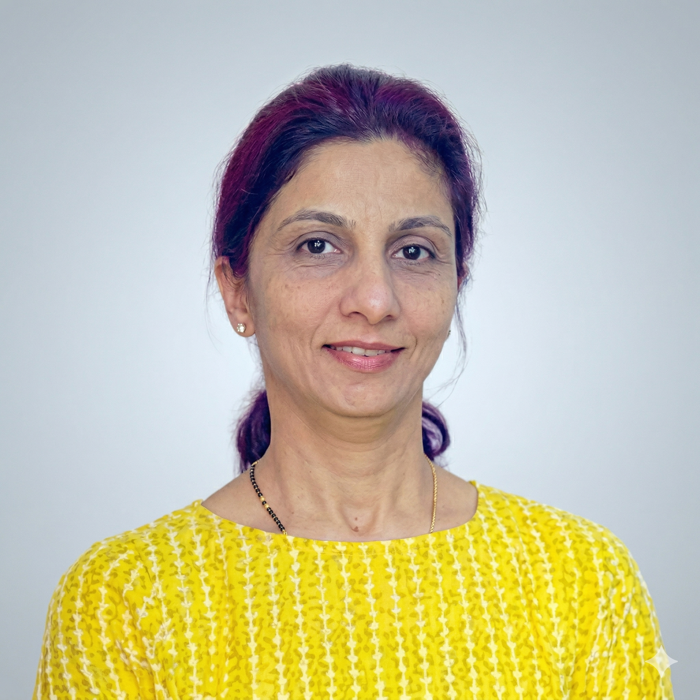
\includegraphics[width=1in,height=1.25in,clip,keepaspectratio]{photo_sapna.png}}]{Sapna Vikram Mewundi}
received the M.Tech. degree in Computer Science and Engineering and the Ph.D. degree from PES University, Bengaluru, India, in 2021. She is an Associate Professor with the Department of Computer Science and Engineering, PES University. Her research interests include digital forensics, computer networks, and cyber security.
\end{IEEEbiography}

\begin{IEEEbiography}[{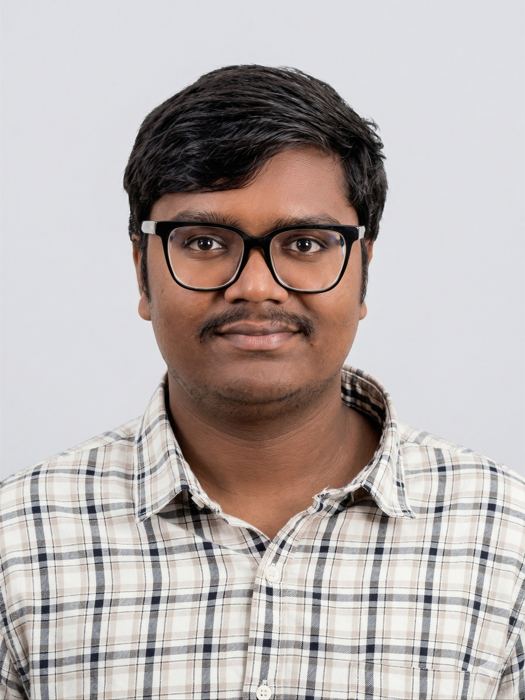
\includegraphics[width=1in,height=1.25in,clip,keepaspectratio]{photo_prajwal.png}}]{Prajwal Chowdary M.}
is a Graduate Researcher in the Department of CSE, PES University, Bengaluru, India. His research interests include post-quantum cryptography, industrial control protocols, and network resilience.
\end{IEEEbiography}

\begin{IEEEbiography}[{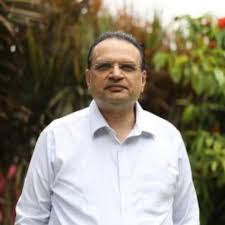
\includegraphics[width=1in,height=1.25in,clip,keepaspectratio]{photo_prasad.jpeg}}]{Prasad B. Honnavalli}
is a Professor with PES University, Bengaluru, India, and Director of the PESU Centre for Information Security, Forensics and Cyber Resilience (C-ISFCR) and the Centre for Internet of Things (C-IoT). His research interests include information, network, and cloud security, cryptography, and the security of IoT, SCADA, and Industry~4.0 systems.
\end{IEEEbiography}

\end{document}
